% !TeX root = report.tex
% 'draft' mode can be used to speed up compilation
\documentclass[twoside,final]{hcmut-report}
\usepackage{longtable}
\usepackage{makecell}
\usepackage{codespace}
\usepackage{enumitem}
\usepackage{listings}
\usepackage{xcolor}
\usepackage{listingsutf8}
\newlist{tabenum}{enumerate}{1}
\setlist[tabenum]{label*=\arabic*.,
                  labelwidth=2em, 
                  leftmargin=2em, 
                  nosep,
                  before=\begin{minipage}[t]{\hsize},
                  after=\end{minipage}}

\usepackage{tabularx}

\usepackage[column=0]{cellspace}
\setlength{\cellspacetoplimit}{\tabcolsep}
\setlength{\cellspacebottomlimit}{\cellspacetoplimit}
\addparagraphcolumntypes{X}

% template %
\newcommand\addrow[2]{#1 & #2\\ \hline}

\newcommand\additemizedrow[2]{#1 &
        \begin{tabenum}
            #2
        \end{tabenum}
        \\ \hline}

% making stuff convenient %
\newcommand\id[1]{\addrow{Use case ID}{#1}}
\newcommand\name[1]{\addrow{Use case Name}{#1}}
\newcommand\actor[1]{\addrow{Actor}{#1}}
\newcommand\udescription[1]{\addrow{Description}{#1}}
\newcommand\precondition[1]{\addrow{Precondition}{#1}}
\newcommand\trigger[1]{\addrow{Trigger}{#1}}
\newcommand\postcondition[1]{\additemizedrow{Postcondition}{#1}}
\newcommand\exceptions[1]{\additemizedrow{Exceptions}{#1}}
\newcommand\nflow[1]{\additemizedrow{Normal flow}{#1}}
\newcommand\aflow[1]{\additemizedrow{Alternative flows}{#1}}
\newenvironment{usecase}{\tabularx{\textwidth}{|0{wl{3cm}}|0{X}|}\hline}{\endtabularx}
\setlength{\parindent}{0em}
\setlength{\parskip}{1em}
% Draft watermark
% https://github.com/callegar/LaTeX-draftwatermark

% Encodings
\usepackage{gensymb,textcomp}

% Better tables
% Wide tables go to https://tex.stackexchange.com/q/332902
\usepackage{array,longtable,multicol,multirow,siunitx,tabularx}

% Better enum
\usepackage{enumitem}

% Graphics
\usepackage{caption,float}

% Add options for figures, like max width, framing, etc.
\usepackage[export]{adjustbox}

% References
% Use \Cref{} instead of \ref{}
\usepackage[nameinlink]{cleveref}

\usepackage{hyperref}

\definecolor{eclipseStrings}{RGB}{42,0.0,255}
\definecolor{eclipseKeywords}{RGB}{127,0,85}
\colorlet{numb}{magenta!60!black}

\lstdefinelanguage{json}{
    basicstyle=\normalfont\ttfamily,
    commentstyle=\color{eclipseStrings}, % style of comment
    stringstyle=\color{eclipseKeywords}, % style of strings
    numbers=left,
    numberstyle=\scriptsize,
    stepnumber=1,
    numbersep=8pt,
    showstringspaces=false,
    breaklines=true,
    frame=lines,
    string=[s]{"}{"},
    comment=[l]{:\ "},
    morecomment=[l]{:"},
    literate=
        *{0}{{{\color{numb}0}}}{1}
         {1}{{{\color{numb}1}}}{1}
         {2}{{{\color{numb}2}}}{1}
         {3}{{{\color{numb}3}}}{1}
         {4}{{{\color{numb}4}}}{1}
         {5}{{{\color{numb}5}}}{1}
         {6}{{{\color{numb}6}}}{1}
         {7}{{{\color{numb}7}}}{1}
         {8}{{{\color{numb}8}}}{1}
         {9}{{{\color{numb}9}}}{1}
}

% FOR DEMONSTRATION PURPOSES, REMOVE IN PRODUCTION
\usepackage{mwe}

% Sub-preambles
% https://github.com/MartinScharrer/standalone

% Configurations
\coursename{CO3029 - KHAI PHÁ DỮ LIỆU}
\reporttype{Báo cáo cuối kì}
\title{Ứng dụng Data Mining trong dự đoán giá nhà}
\advisor{& Đỗ Thanh Thái &}
\stuname{%
	& Võ Ngọc Tú & ID 2213857 \\
	& Trần Tuấn Kiệt & ID 2311787 \\
	& Bùi Hà Hải & ID 2310862 \\
	& \multicolumn{2}{c}{\textbf{Link GitHub:} \href{https://github.com/LouisVo3105/Data-Mining-252.git}{Data-Mining-252}} \\
}


% Allow page breaks inside align* environment
%\allowdisplaybreaks{}

% Makes a lot of things blue, avoid at all costs
%\everymath{\color{blue}}

% Set depth of numbering for counters
\AtBeginDocument{\counterwithin{lstlisting}{section}}

% Rename some sections
%\AtBeginDocument{\renewcommand*{\contentsname}{Contents}}
%\AtBeginDocument{\renewcommand*{\refname}{References}}
%\AtBeginDocument{\renewcommand*{\bibname}{References}}

% Custom commands
%\newcommand*\mean[1]{\bar{#1}}

\begin{document}
\coverpage%

\section*{Phân công công việc}
\newcounter{memberrowno}
\setcounter{memberrowno}{0}
\begin{center}
 \begin{tabular}{>{\stepcounter{memberrowno}\thememberrowno}llccc}
   \toprule
   \multicolumn{1}{c}{\textbf{No.}} & \textbf{Họ và Tên} & \textbf{MSSV} & \textbf{Công việc} & \textbf{Phần trăm}\\
   \midrule
   & Trần Tuấn Kiệt & 2311787 & \makecell{Tiền xử lý và phân tích dữ liệu \\ Đánh giá và so sánh các mô hình} & 100\%\\
   \midrule
   & Võ Ngọc Tú & 2213857 & \makecell{MLP Neural network \\ XGBoost Regression} &  100\%\\
   \midrule
   & Bùi Hà Hải & 2310862 & \makecell{ Random Forest Regression\\ Linear Regression } & 100\% \\               
   \bottomrule
 \end{tabular}
\end{center}
\clearpage

\tableofcontents
\listoffigures
\listoftables

\clearpage
\section{Tiền xử lý dữ liệu}
\subsection{Tổng quan về dữ liệu}

\hspace{10pt}
File dữ liệu đầu vào được nhóm quyết định chọn trên nền tảng Kaggle có tên \textbf{Housing.csv} tại 
\href{https://www.kaggle.com/datasets/yasserh/housing-prices-dataset}{housing-prices-dataset}. Bộ dữ liệu gồm các thông tin như giá bất động sản, diện tích, số phòng ngủ, số phòng tắm, v.v. Mục tiêu của bài tập lớn này là tìm ra mối quan hệ giữa giá bất động sản và các đặc tính của căn nhà.\\
\hspace{10pt}

Bộ dữ liệu bao gồm 545 mẫu, mỗi mẫu đại diện cho một căn nhà với các cột đặc tính sau:
\begin{itemize}
	\item \textbf{price}: giá bán của căn nhà (đơn vị: USD)
	\item area: diện tích của căn nhà (feet vuông)
	\item bedrooms: số lượng phòng ngủ
	\item bathrooms: số lượng phòng tắm
	\item mainroad: có nằm ở mặt tiền hay không
	\item guestroom: có phòng khách hay không
	\item basement: có tầng hầm hay không
	\item hotwaterheating: có máy nước nóng hay không
	\item airconditioning: có điều hòa hay không
	\item parking: số lượng bãi đậu xe
	\item prefarea: thuộc khu vực ưu tiên hay không
	\item furnishingstatus: tình trạng nội thất (unfurnished, semi-furnished, furnished)
\end{itemize}

\subsection{Xử lý dữ liệu}

\subsubsection{Đọc dữ liệu}

\hspace{10pt}
Sau khi đọc dữ liệu, ta lưu vào Pandas DataFrame.\\
\hspace{10pt}

Hình bên dưới minh họa 5 dòng đầu trong bộ dữ liệu để có cái nhìn tổng quát hơn.
\begin{figure}[h]
	\centering
	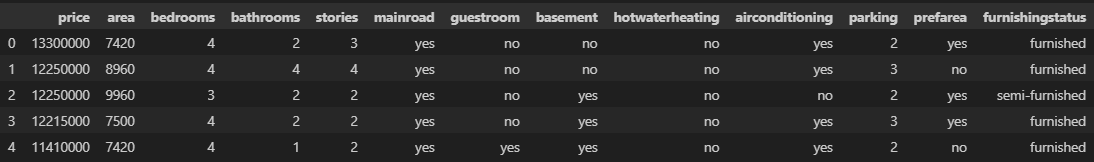
\includegraphics[width=\textwidth]{chapters/Preprocessing/images/demo_data.png}
	\caption{Thông tin cơ bản về tập dữ liệu}
\end{figure}

\subsubsection{Kiểm tra và xử lý dữ liệu khuyết}
\hspace{10pt}
Để kiểm tra dữ liệu khuyết và dữ liệu trùng trong tập dữ liệu, ta sử dụng 2 lệnh: 
data.isnull().sum() và data.duplicated().sum() để thống kê lại tổng số dữ liệu khuyết và dữ liệu trùng lặp trên từng cột:
\begin{figure}[h]
	\centering
	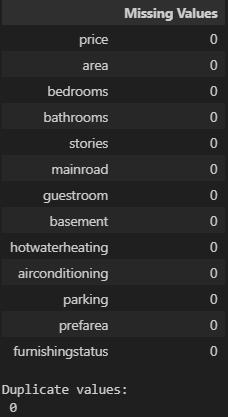
\includegraphics[width=0.3\textwidth]{chapters/Preprocessing/images/miss_value.png}
	\caption{Thống kê dữ liệu khuyết và trùng lặp}
\end{figure}

Dựa vào hình trên, ta có thể thấy rằng không có giá trị khuyết và giá trị trùng lặp tồn tại trong tập dữ liệu. Do đó, không cần xử lý dữ liệu khuyết cũng như dữ liệu trùng lặp.

\subsubsection{Xử lý dữ liệu phân loại}
\hspace{10pt}
Để kiểm tra sự tồn tại của dữ liệu phân loại trong tập dữ liệu, ta sử dụng lệnh \texttt{data.dtypes} nhằm thống kê các kiểu dữ liệu của các đặc trưng.

\begin{figure}[H]
	\centering
	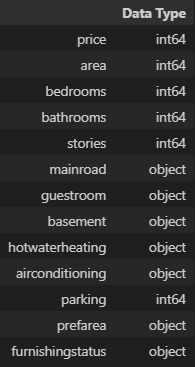
\includegraphics[width=0.3\textwidth]{chapters/Preprocessing/images/initial_dtype.png}
	\caption{Thống kê kiểu dữ liệu}
\end{figure}
\hspace{10pt}

Dựa vào hình, ta có thể thấy rằng các cột có kiểu dữ liệu là \texttt{object} gồm: \texttt{mainroad}, \texttt{guestroom}, \texttt{basement}, \texttt{hotwaterheating}, \texttt{airconditioning}, \texttt{prefarea}, và \texttt{furnishingstatus} -- đây là các cột chứa giá trị phân loại. Ta áp dụng kỹ thuật One-Hot Encoding để chuyển đổi các cột này thành các giá trị nhị phân tương ứng với từng loại giá trị. Ngoài ra, ta sẽ sử dụng tham số \texttt{drop\_first=True} để tránh trường hợp đa cộng tuyến. Sau khi xử lý, tập dữ liệu sẽ được chuyển hóa thành như sau:
\begin{figure}[H]
	\centering
	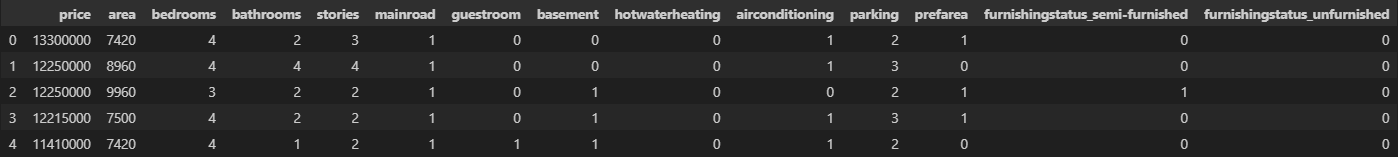
\includegraphics[width=\textwidth]{chapters/Preprocessing/images/dtype.png}
	\caption{Thống kê kiểu dữ liệu sau khi phân loại}
\end{figure}
\section{Phân tích dữ liệu}
\begin{figure}[H]
	\centering
	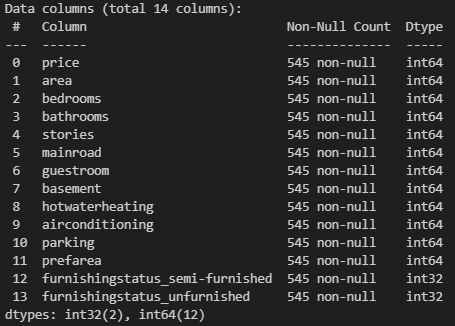
\includegraphics[width=0.7\textwidth]{chapters/Preprocessing/images/info_data.png}
	\caption{Tập dữ liệu sau khi xử lý}
\end{figure}
\hspace{10pt}

Trước khi phân tích dữ liệu, ta phân tích tổng quan dữ liệu sau tiền xử lý. Ta sử dụng \texttt{df.info()}. Dựa vào Hình 3.1, ta có thể rút ra được rằng:

\begin{itemize}
	\item Dữ liệu bao gồm 545 mẫu.
	\item Ở mỗi cột dữ liệu đều đếm được 545 dòng dữ liệu không rỗng.
	\item Tất cả 14 cột đều có kiểu \texttt{int64}.
\end{itemize}

Trong đó, biến dữ liệu được chia thành hai loại: biến liên tục và biến rời rạc.

\begin{itemize}
	\item Biến liên tục: là biến có thể nhận vô số giá trị $\rightarrow$ \texttt{area}.
	
	\item Biến rời rạc: là biến chỉ có thể nhận hữu hạn các giá trị riêng biệt $\rightarrow$ 
	\texttt{bedrooms}, \texttt{bathrooms}, \texttt{stories}, \texttt{parking}, 
	\texttt{mainroad\_yes}, \texttt{guestroom\_yes}, \texttt{basement\_yes}, 
	\texttt{hotwaterheating\_yes}, \texttt{airconditioning\_yes}, \texttt{prefarea\_yes}, 
	\texttt{furnishingstatus\_semi-furnished}, và 
	\texttt{furnishingstatus\_unfurnished}.
\end{itemize}

\section{Kiểm tra phân bố và outliers của "price"}

\hspace{10pt}
Trước khi phân tích sự tương quan của các thuộc tính, ta cần kiểm tra sự phân bố của
"price":
\begin{figure}[H]
	\centering
	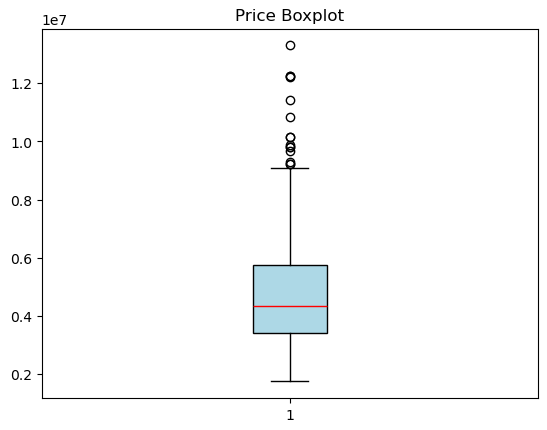
\includegraphics[width=0.7\textwidth]{chapters/Preprocessing/images/price_ouliers.png}
	\caption{Giá trị outliers của "price"}
\end{figure}
\begin{figure}[H]
	\centering
	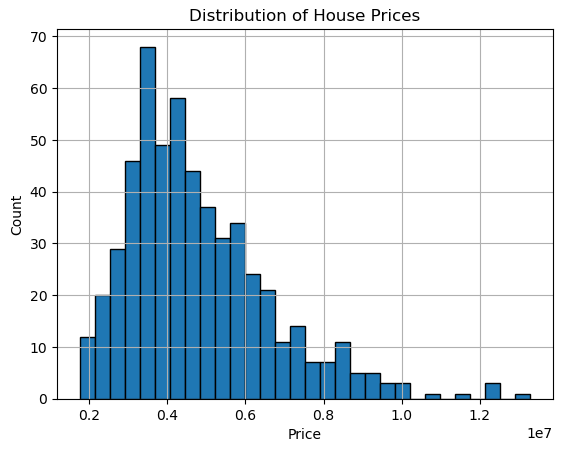
\includegraphics[width=0.7\textwidth]{chapters/Preprocessing/images/distribution.png}
	\caption{Biểu đồ phân bố "price"}
\end{figure}
\textbf{Đánh giá chung:} Biến \texttt{price} có phân phối lệch phải (right-skewed) rõ rệt, với phần lớn dữ liệu tập trung ở phân khúc giá thấp và trung bình (khoảng $3 \times 10^6$ đến $6 \times 10^6$). Cả hai biểu đồ đều xác nhận sự hiện diện của nhiều giá trị ngoại lệ (outliers) phía cao, cho thấy thị trường tồn tại một số bất động sản có giá trị đột biến so với mặt bằng chung. Đặc điểm này gợi ý rằng việc áp dụng biến đổi logarit có thể cần thiết để đưa dữ liệu về phân phối chuẩn hơn trước khi đưa vào các mô hình dự báo.
\subsection{Ma trận tương quan của các biến}

Để phân tích mối quan hệ giữa các đặc trưng trong tập dữ liệu, ta sử dụng ma trận tương quan. Ma trận này biểu diễn mức độ tương quan tuyến tính giữa các cặp thuộc tính, với giá trị nằm trong khoảng từ $-1$ đến $1$. Trong đó:

\begin{itemize}
	\item Giá trị gần $1$ biểu thị mối tương quan thuận mạnh.
	\item Giá trị gần $-1$ biểu thị mối tương quan nghịch mạnh.
	\item Giá trị gần $0$ biểu thị mối tương quan yếu hoặc không tồn tại.
\end{itemize}
\begin{figure}[H]
	\centering
	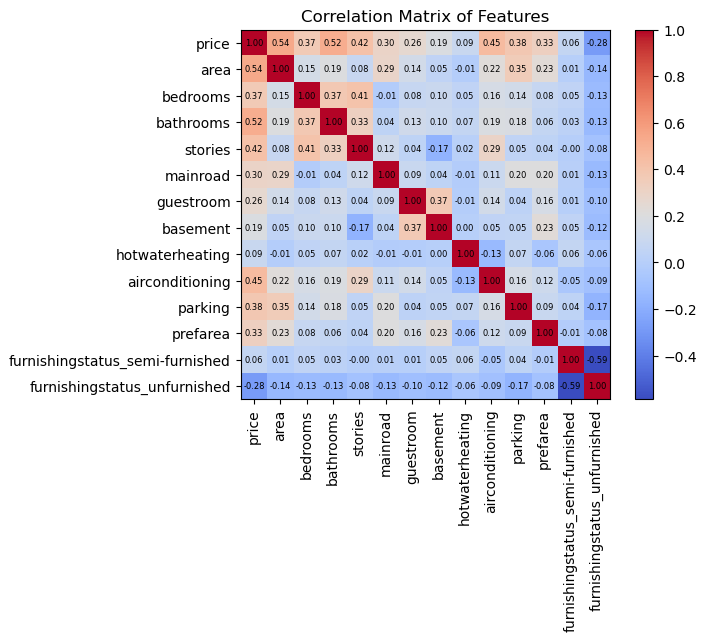
\includegraphics[width=0.9\textwidth]{chapters/Preprocessing/images/correlation.png}
	\caption{Biểu đồ tương quan giữa các biến}
\end{figure}
\hspace{10pt}

Dựa vào hình, ta nhận thấy một số biến có mối tương quan đáng kể với biến mục tiêu \texttt{price}. Cụ thể, các biến như \texttt{area} ($r = 0.54$), \texttt{bathrooms} ($r = 0.52$), \texttt{stories} ($r = 0.45$), và \texttt{airconditioning} ($r = 0.42$) có mức tương quan khá mạnh, cho thấy chúng có ảnh hưởng rõ rệt đến giá nhà. 

Bên cạnh đó, các biến như \texttt{bedrooms}, \texttt{parking}, \texttt{mainroad} và \texttt{prefarea} có hệ số tương quan ở mức trung bình ($0.30 \leq r < 0.4$), vẫn có thể được xem xét trong quá trình xây dựng mô hình.

Ngược lại, các đặc trưng như \texttt{basement}, \texttt{guestroom}, \texttt{hotwaterheating} và \texttt{furnishingstatus} có tương quan yếu hoặc gần như không có tương quan với giá nhà ($r < 0.2$), thậm chí có một số biến như \texttt{mainroad\_no} thể hiện mối quan hệ ngược chiều ($r = -0.28$).

\subsection{Trực quan hóa dữ liệu}

Trực quan hóa dữ liệu sẽ giúp ta hiểu rõ hơn về phân bố, xu hướng và mối quan hệ giữa các biến và biến \texttt{price}.

\begin{itemize}
	\item Biến liên tục: ta sử dụng boxplot để biểu thị sự phân bố của nó và scatterplot để
\end{itemize}
biểu hiện phân bố theo \texttt{price}

\begin{itemize}
	\item Biến rời rạc: ta sử dụng barplot để biểu thị sự phân bố của nó và boxplot để biểu hiện phân bố theo \texttt{price}
\end{itemize}

\subsubsection{Biến \texttt{area}}
\begin{figure}[H]
	\centering
	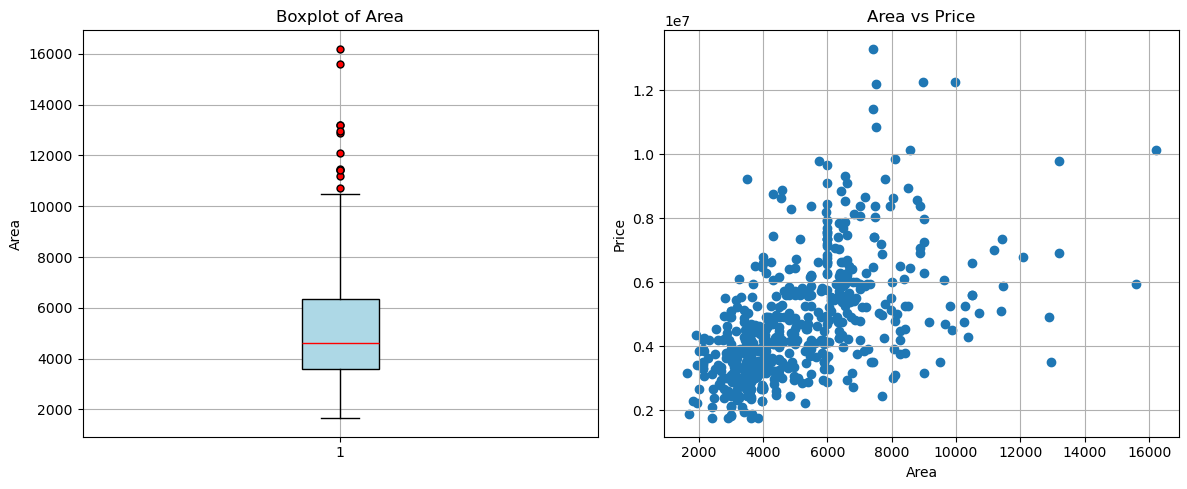
\includegraphics[width=\textwidth]{chapters/Preprocessing/images/area.png}
	\caption{Biến "area"}
\end{figure}

\subsubsection{Biến "bedrooms"}
\begin{figure}[H]
	\centering
	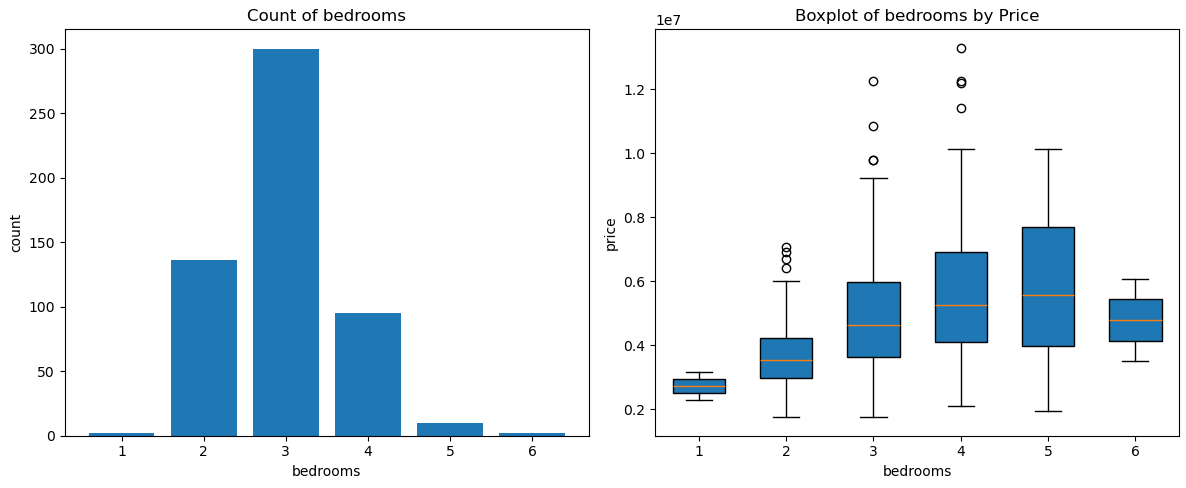
\includegraphics[width=\textwidth]{chapters/Preprocessing/images/bedroom.png}
	\caption{Biến "bedrooms"}
\end{figure}

\subsubsection{Biến "bathrooms"}
\begin{figure}[H]
	\centering
	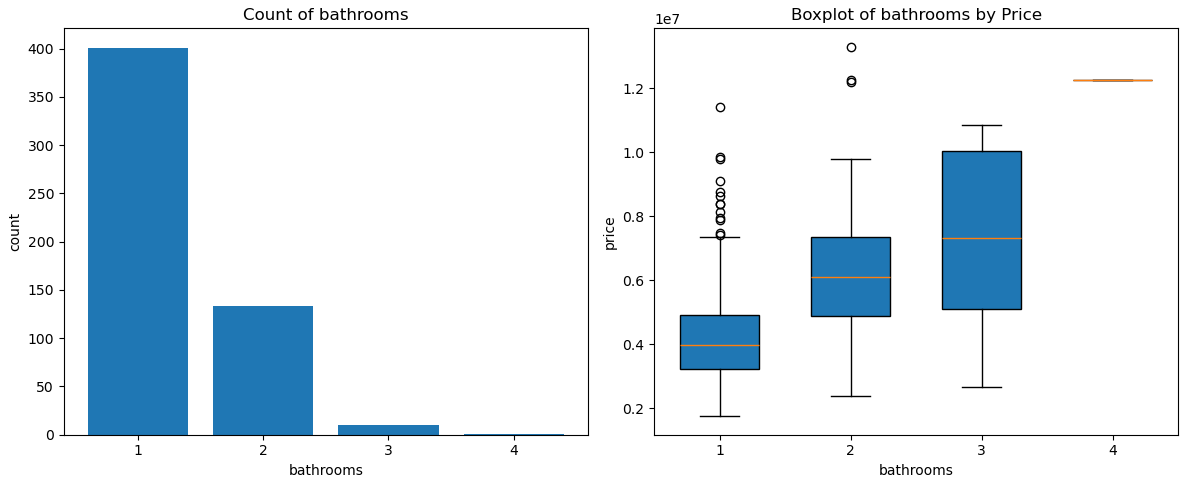
\includegraphics[width=\textwidth]{chapters/Preprocessing/images/bathroom.png}
	\caption{Biến "bathrooms"}
\end{figure}

\subsubsection{Biến "stories"}
\begin{figure}[H]
	\centering
	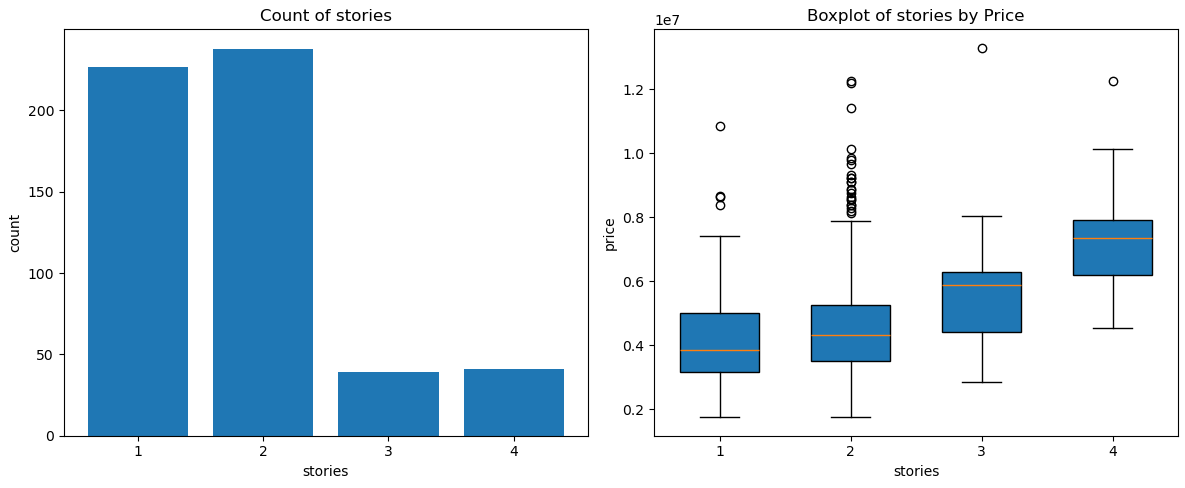
\includegraphics[width=\textwidth]{chapters/Preprocessing/images/storie.png}
	\caption{Biến "stories"}
\end{figure}

\subsubsection{Biến "parking"}
\begin{figure}[H]
	\centering
	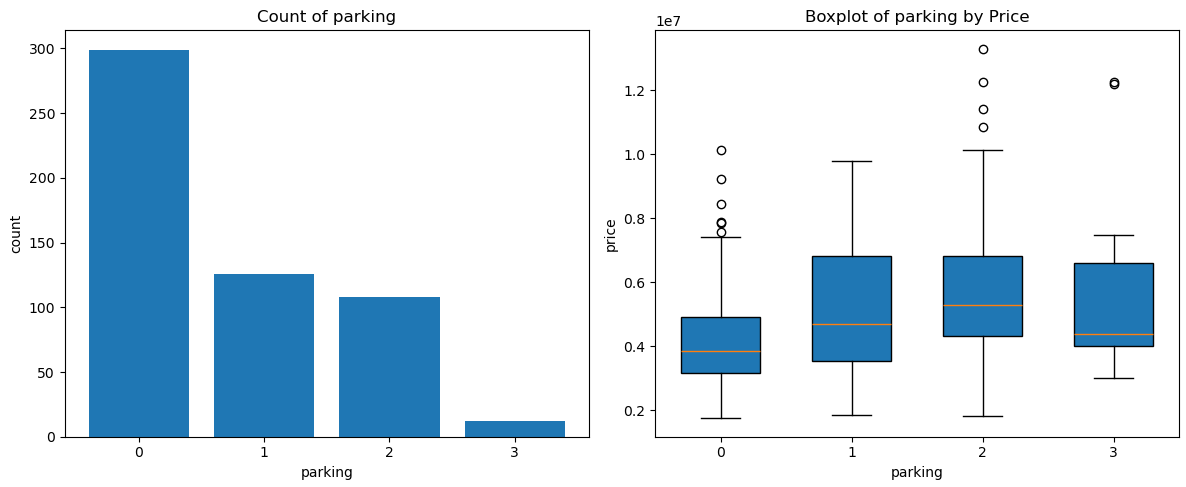
\includegraphics[width=\textwidth]{chapters/Preprocessing/images/parking.png}
	\caption{Biến "parking"}
\end{figure}

\subsubsection{Biến "mainroad"}
\begin{figure}[H]
	\centering
	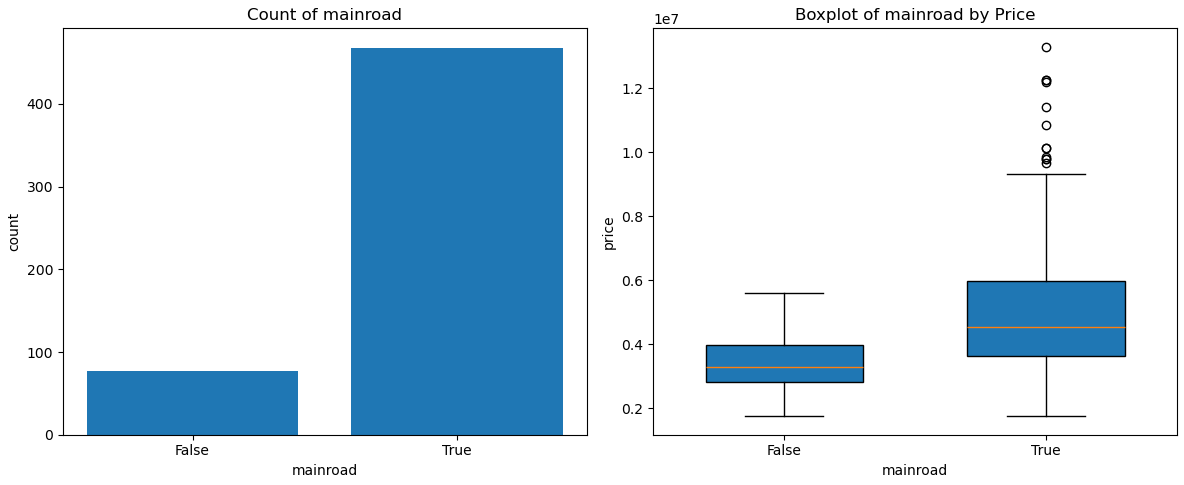
\includegraphics[width=\textwidth]{chapters/Preprocessing/images/mainroad.png}
	\caption{Biến "mainroad"}
\end{figure}

\subsubsection{Biến "guestroom"}
\begin{figure}[H]
	\centering
	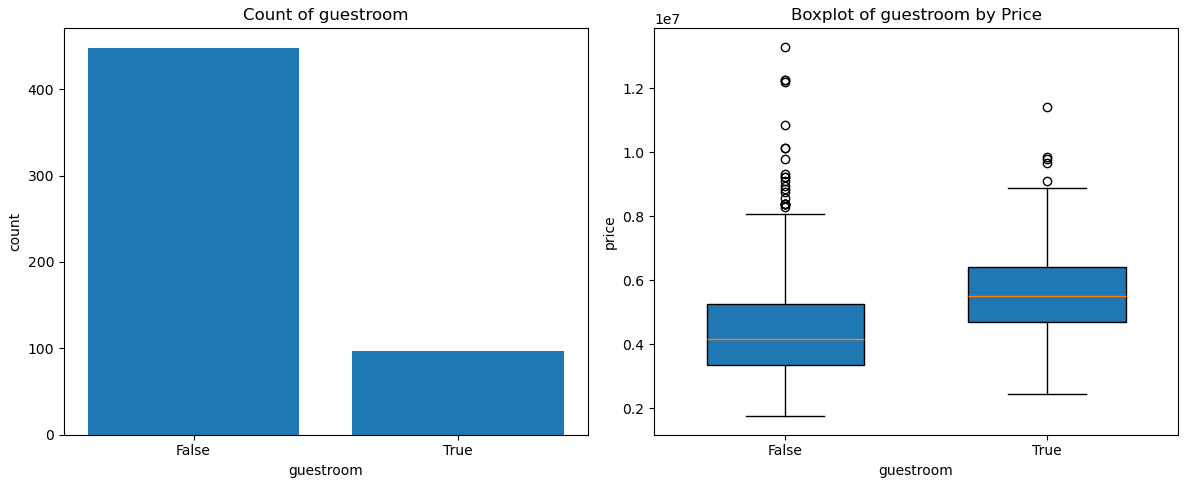
\includegraphics[width=\textwidth]{chapters/Preprocessing/images/guestroom.png}
	\caption{Biến "guestroom"}
\end{figure}

\subsubsection{Biến "basement"}
\begin{figure}[H]
	\centering
	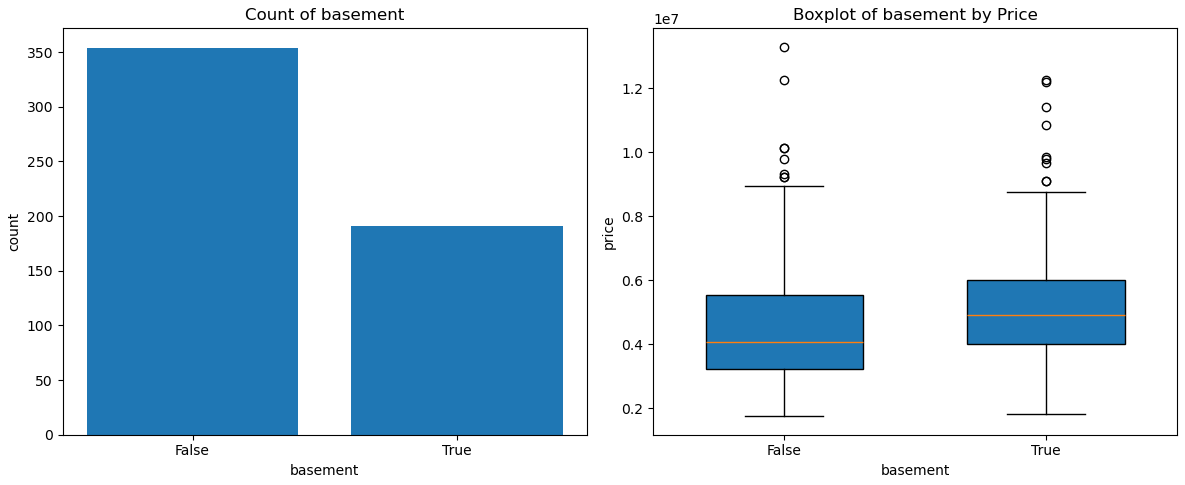
\includegraphics[width=\textwidth]{chapters/Preprocessing/images/basement.png}
	\caption{Biến "basement"}
\end{figure}

\subsubsection{Biến "hotwaterheating"}
\begin{figure}[H]
	\centering
	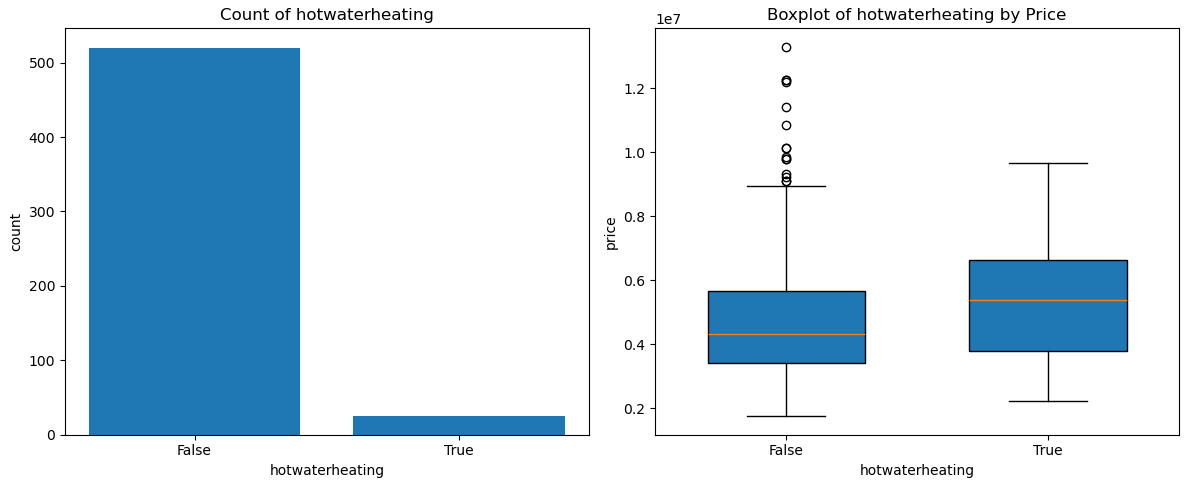
\includegraphics[width=\textwidth]{chapters/Preprocessing/images/hotwaterheating.png}
	\caption{Biến "hotwaterheating"}
\end{figure}

\subsubsection{Biến "airconditioning"}
\begin{figure}[H]
	\centering
	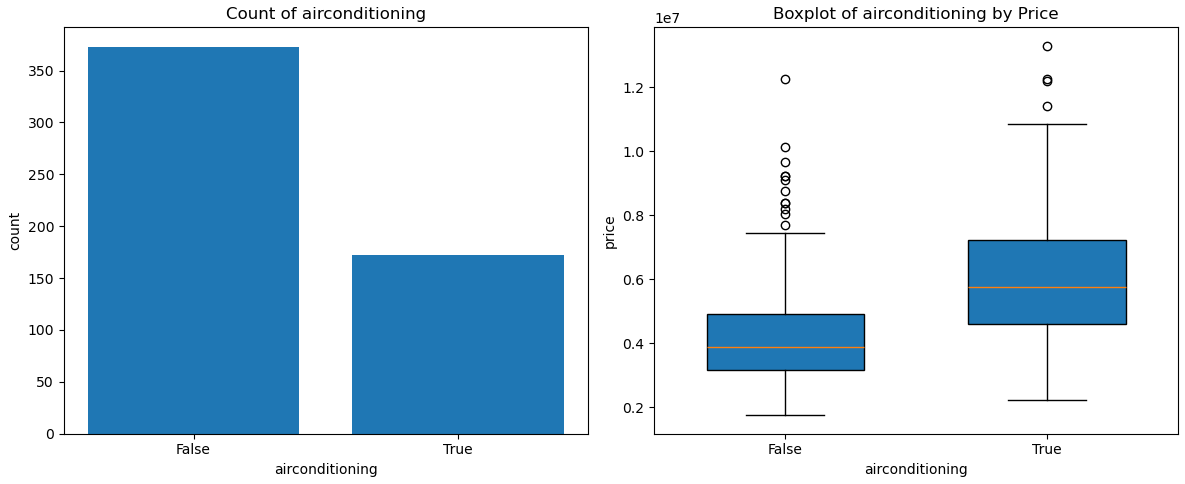
\includegraphics[width=\textwidth]{chapters/Preprocessing/images/airconditioning.png}
	\caption{Biến "airconditioning"}
\end{figure}

\subsubsection{Biến "prefarea"}
\begin{figure}[H]
	\centering
	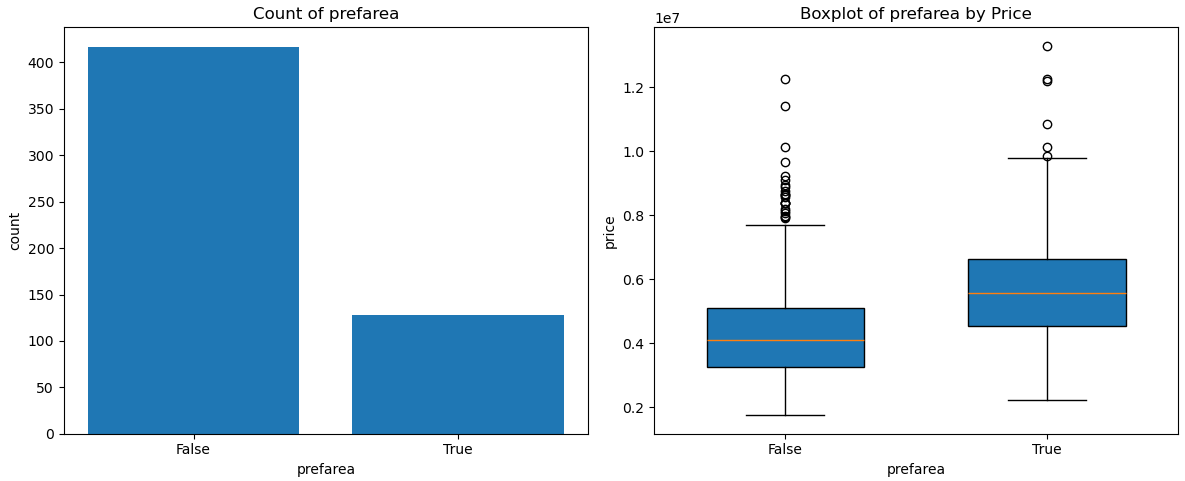
\includegraphics[width=\textwidth]{chapters/Preprocessing/images/prefarea.png}
	\caption{Biến "prefarea"}
\end{figure}

\subsubsection{Biến "furnishingstatus\_semi-furnished"}
\begin{figure}[H]
	\centering
	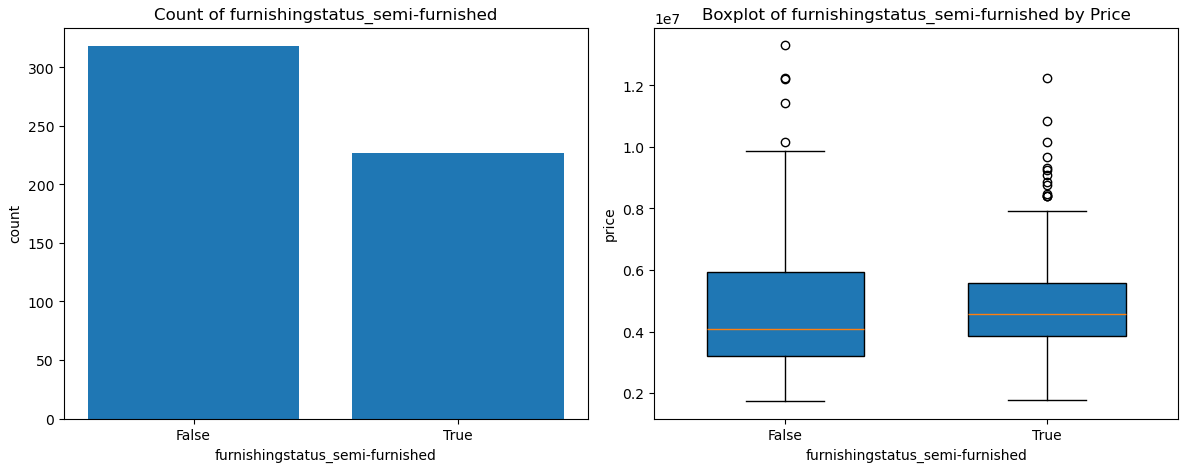
\includegraphics[width=\textwidth]{chapters/Preprocessing/images/semi-fur.png}
	\caption{Biến "furnishingstatus\_semi-furnished"}
\end{figure}

\subsubsection{Biến "furnishingstatus\_unfurnished"}
\begin{figure}[H]
	\centering
	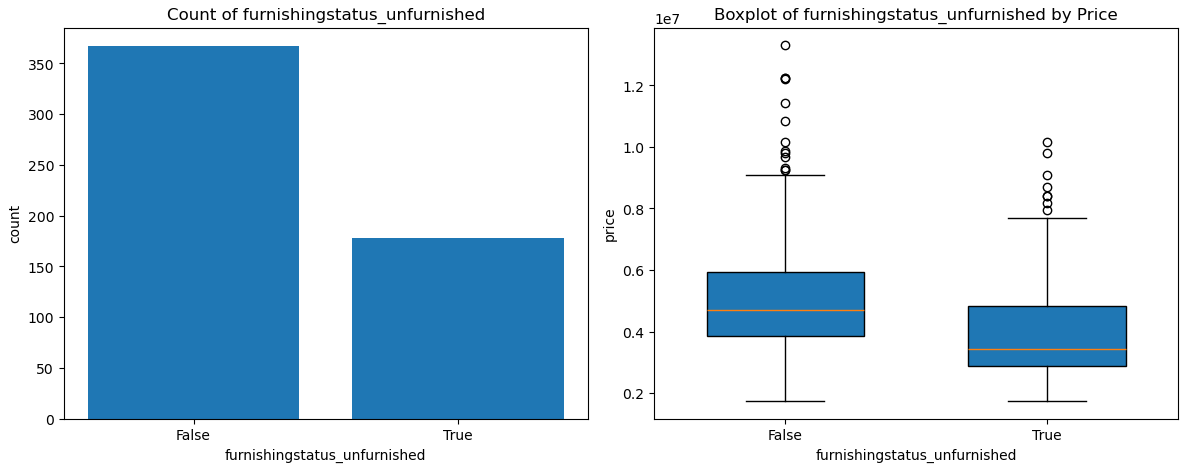
\includegraphics[width=\textwidth]{chapters/Preprocessing/images/unfur.png}
	\caption{Biến "furnishingstatus\_unfurnished"}
\end{figure}
\section{Phương pháp}

\subsection{Hồi quy tuyến tính}

Hồi quy tuyến tính (Linear Regression) là một trong những phương pháp cơ bản và phổ biến nhất trong \textit{Data Mining} và \textit{Machine Learning}, được sử dụng để mô hình hóa mối quan hệ giữa một biến phụ thuộc và một hoặc nhiều biến độc lập. Mục tiêu của mô hình là tìm ra một hàm tuyến tính tốt nhất để dự đoán giá trị đầu ra dựa trên dữ liệu đầu vào.

Giả định cốt lõi của hồi quy tuyến tính là tồn tại mối quan hệ tuyến tính giữa các biến, tức là đầu ra có thể được biểu diễn dưới dạng tổ hợp tuyến tính của các biến đầu vào.

\subsubsection*{Nguyên lý hoạt động:}

\begin{itemize}
    \item \textbf{Hồi quy tuyến tính đơn (một biến đầu vào):}
    \[
        y = wx + b
    \]
    Trong đó:
    \begin{itemize}
        \item $y$: biến phụ thuộc (giá trị cần dự đoán)
        \item $x$: biến độc lập
        \item $w$: hệ số hồi quy (trọng số)
        \item $b$: hệ số chệch (bias/intercept)
    \end{itemize}
    
    \item \textbf{Hồi quy tuyến tính đa biến:}
    \[
        y = w_1x_1 + w_2x_2 + \cdots + w_nx_n + b = \mathbf{w}^T \mathbf{x} + b
    \]
    Với:
    \[
        \mathbf{x} = [x_1, x_2, \ldots, x_n]^T,\quad 
        \mathbf{w} = [w_1, w_2, \ldots, w_n]^T
    \]
\end{itemize}

Để đánh giá chất lượng mô hình, hàm mất mát phổ biến được sử dụng là \textbf{Mean Squared Error (MSE)}:

\[
    \text{MSE} = \frac{1}{m} \sum_{i=1}^{m} \left( y^{(i)} - \hat{y}^{(i)} \right)^2
\]

Trong đó:
\begin{itemize}
    \item $m$: số lượng mẫu
    \item $y^{(i)}$: giá trị thực tế
    \item $\hat{y}^{(i)}$: giá trị dự đoán
\end{itemize}

Mục tiêu của quá trình huấn luyện là tìm bộ tham số $\mathbf{w}, b$ sao cho MSE được tối thiểu hóa. Điều này thường được thực hiện thông qua các phương pháp tối ưu như \textit{Gradient Descent} hoặc nghiệm giải tích (\textit{Normal Equation}).

\subsubsection*{Ưu điểm và hạn chế:}

\begin{itemize}
    \item \textbf{Ưu điểm:}
    \begin{itemize}
        \item Đơn giản, dễ triển khai và huấn luyện nhanh
        \item Dễ diễn giải, cho phép hiểu rõ ảnh hưởng của từng đặc trưng
        \item Hoạt động tốt với dữ liệu có quan hệ tuyến tính
    \end{itemize}
    
    \item \textbf{Hạn chế:}
    \begin{itemize}
        \item Không mô hình hóa được quan hệ phi tuyến
        \item Nhạy cảm với outliers
        \item Có thể bị underfitting nếu dữ liệu phức tạp
    \end{itemize}
\end{itemize}

Trong bài toán dự đoán giá nhà, hồi quy tuyến tính là một mô hình cơ sở (\textit{baseline}) hiệu quả, giúp mô tả mối quan hệ giữa các đặc trưng như diện tích, số phòng, vị trí và giá trị bất động sản. Mặc dù đơn giản, mô hình vẫn cung cấp khả năng dự đoán tốt và đặc biệt hữu ích trong việc phân tích mức độ ảnh hưởng của từng yếu tố.

\subsection{Random Forest}

Random Forest là một phương pháp học máy thuộc nhóm \textit{Ensemble Learning}, được đề xuất nhằm cải thiện độ chính xác và khả năng tổng quát hóa của mô hình bằng cách kết hợp nhiều cây quyết định (\textit{Decision Trees}). Phương pháp này có thể áp dụng cho cả bài toán phân loại và hồi quy.

Trong bài toán hồi quy (Random Forest Regression), mô hình dự đoán giá trị liên tục bằng cách lấy trung bình kết quả từ nhiều cây hồi quy.

\subsubsection*{Nguyên lý hoạt động:}

Giả sử có $T$ cây hồi quy \( f_1(x), f_2(x), \ldots, f_T(x) \). Mỗi cây được huấn luyện độc lập trên một tập dữ liệu con được tạo ra bằng phương pháp \textbf{Bootstrap Sampling} từ tập dữ liệu gốc $D$:

\[
D_t \sim \text{Bootstrap}(D), \quad t = 1, 2, \ldots, T
\]

Ngoài ra, tại mỗi nút của cây, chỉ một tập con ngẫu nhiên các đặc trưng \( \mathcal{F}_t \subseteq \mathcal{F} \) được sử dụng để tìm điểm chia tối ưu. Điều này giúp tăng tính đa dạng giữa các cây và giảm tương quan giữa chúng.

Việc phân chia dữ liệu tại mỗi nút dựa trên tiêu chí giảm thiểu sai số, thường sử dụng \textbf{Sum of Squared Errors (SSE)}:

\[
\text{SSE} = \sum_{i \in S} \left( y^{(i)} - \bar{y}_S \right)^2
\]

Trong đó:
\[
\bar{y}_S = \frac{1}{|S|} \sum_{i \in S} y^{(i)}
\]

Cây sẽ tiếp tục phát triển cho đến khi đạt các điều kiện dừng như:
\begin{itemize}
    \item Độ sâu tối đa
    \item Số mẫu tối thiểu tại một nút
    \item Mức giảm sai số không còn đáng kể
\end{itemize}

Sau khi huấn luyện, dự đoán cuối cùng của mô hình được tính bằng trung bình các dự đoán từ tất cả các cây:

\[
\hat{y} = \frac{1}{T} \sum_{t=1}^{T} f_t(x)
\]

\begin{itemize}
    \item $T$: số lượng cây
    \item $f_t(x)$: dự đoán của cây thứ $t$
    \item $\hat{y}$: giá trị dự đoán cuối cùng
\end{itemize}

\subsubsection*{Ưu điểm và hạn chế:}

\begin{itemize}
    \item \textbf{Ưu điểm:}
    \begin{itemize}
        \item Mô hình hóa tốt các quan hệ phi tuyến phức tạp
        \item Giảm overfitting nhờ cơ chế ensemble
        \item Ít nhạy cảm với nhiễu và outliers
        \item Tự động đánh giá mức độ quan trọng của đặc trưng
    \end{itemize}
    
    \item \textbf{Hạn chế:}
    \begin{itemize}
        \item Chi phí tính toán cao hơn hồi quy tuyến tính
        \item Khó diễn giải hơn (black-box hơn)
        \item Mô hình lớn, tốn bộ nhớ
    \end{itemize}
\end{itemize}

Trong bài toán dự đoán giá nhà, Random Forest cho phép mô hình hóa các mối quan hệ phi tuyến giữa các yếu tố như diện tích, vị trí địa lý, tiện ích xung quanh và giá trị bất động sản. Nhờ khả năng tổng hợp nhiều cây quyết định, mô hình mang lại độ chính xác cao và khả năng tổng quát hóa tốt hơn so với các phương pháp tuyến tính.


\subsection{XGBoost}
XGBoost (Extreme Gradient Boosting) là một thuật toán học máy mạnh mẽ thuộc nhóm ensemble learning, cụ thể là phương pháp boosting. Nó được thiết kế để tối ưu hiệu năng và tốc độ khi huấn luyện mô hình cây quyết định.
\subsubsection*{Nguyên lý hoạt động:}
XGBoost xây dựng mô hình bằng cách kết hợp nhiều cây quyết định theo từng vòng lặp. Mỗi cây mới được huấn luyện nhằm sửa lỗi của cây trước đó, giúp mô hình học tốt hơn theo thời gian.

\subsubsection*{1. Hàm mục tiêu}

Ở vòng boosting thứ \( t \), mô hình XGBoost tối ưu hàm mục tiêu sau:
\[
\mathcal{L}^{(t)} = \sum_{i=1}^{n} l(y_i, \hat{y}_i^{(t-1)} + f_t(x_i)) + \Omega(f_t)
\]

Trong đó:
\begin{itemize}
	\item \( l \): hàm mất mát (thường dùng MSE: \( l(y, \hat{y}) = (y - \hat{y})^2 \))
	\item \(\hat{y_i}^{(t-1)}\): dự đoán của mô hình tại bước t - 1
	\item \(f_t\): cây quyết định mới tại bước t
	\item \( \Omega(f_t) \): thành phần regularization giúp chống overfitting
\end{itemize}

\[\Omega(f)f_t  = \gamma T + \frac{1}{2} \lambda \sum_{j=1}^{T} w_j^2 \]

Trong đó:
\begin{itemize}
	\item \(T\): số lá của cây
	\item \(w_j\): trọng số lá thứ \(j\)
	\item \(\gamma, \lambda\): hệ số điều chỉnh độ phức tạp mô hình
\end{itemize}
\subsubsection*{2. Xấp xỉ Taylor bậc hai}

XGBoost sử dụng xấp xỉ Taylor bậc hai để làm trơn hàm mất mát:

\[
\mathcal{L}^{(t)} \approx \sum_{i=1}^{n} \left[ g_i f_t(x_i) + \frac{1}{2} h_i f_t^2(x_i) \right] + \Omega(f_t)
\]

Trong đó:
- \( g_i = \frac{\partial l(y_i, \hat{y}_i^{(t-1)})}{\partial \hat{y}_i^{(t-1)}} \) (đạo hàm bậc 1)
- \( h_i = \frac{\partial^2 l(y_i, \hat{y}_i^{(t-1)})}{\partial (\hat{y}_i^{(t-1)})^2} \) (đạo hàm bậc 2)

\subsubsection*{3. Tính giá trị tối ưu tại mỗi lá}

Với mỗi lá \( j \), tập mẫu thuộc lá là \( I_j \). Tổng gradient và hessian tại lá:

\[
G_j = \sum_{i \in I_j} g_i, \quad H_j = \sum_{i \in I_j} h_i
\]

Giá trị đầu ra tối ưu tại lá:

\[
w_j^* = -\frac{G_j}{H_j + \lambda}
\]

Giá trị hàm mục tiêu tại điểm cực tiểu:

\[
\mathcal{L}^{(t)} = -\frac{1}{2} \sum_{j=1}^{T} \frac{G_j^2}{H_j + \lambda} + \gamma T
\]

\subsubsection*{Quá trình huấn luyện:}
Quá trình huấn luyện XGBoost bao gồm các bước chính sau:

\begin{itemize}
	\item[1. ] \textbf{Khởi tạo mô hình:} Dự đoán ban đầu là giá trị trung bình (cho hồi quy) hoặc xác suất (cho phân loại).
	\item[2.] \textbf{Tính toán gradient và hessian:} Các gradient (\( g_i \)) và hessian (\( h_i \)) được tính cho mỗi mẫu dựa trên hàm mất mát.
	\item[3.] \textbf{Xây dựng cây quyết định:} Mỗi cây mới được xây dựng để tối ưu hóa hàm mất mát với việc sử dụng gradient và hessian.
	\item[4.] \textbf{Cập nhật dự đoán:} Dự đoán của mô hình được cập nhật bằng cách cộng thêm giá trị từ cây mới.
	\item[5.] \textbf{Regularization:} Thành phần regularization giúp kiểm soát độ phức tạp của mô hình và ngăn ngừa overfitting.
	\item[6.] \textbf{Lặp lại quá trình:} Các bước trên được lặp lại cho đến khi đạt số vòng lặp tối đa hoặc không còn cải thiện đáng kể.
\end{itemize}

XGBoost là một lựa chọn mạnh mẽ cho bài toán hồi quy dự đoán giá nhà nhờ vào khả năng xử lý các mối quan hệ phi tuyến tính phức tạp trong dữ liệu. Mô hình này sử dụng kỹ thuật boosting, giúp tăng cường độ chính xác qua từng vòng lặp bằng cách học từ các sai sót của các cây quyết định trước đó. Điều này giúp XGBoost cải thiện hiệu suất so với mô hình hồi quy tuyến tính, vốn chỉ phù hợp với mối quan hệ tuyến tính giữa các đặc trưng và giá trị dự đoán.

Khác biệt với Random Forest, XGBoost không chỉ tạo ra nhiều cây quyết định độc lập mà còn tập trung vào việc tối ưu hóa mỗi cây dựa trên gradient của hàm mất mát, giúp giảm sai số một cách hiệu quả. Mặc dù Random Forest có thể xử lý các mối quan hệ phi tuyến tính, nhưng XGBoost thường cho kết quả tốt hơn nhờ vào khả năng tối ưu hóa liên tục và điều chỉnh chính xác hơn qua mỗi vòng huấn luyện.

\subsection{GridSearchCV} 
GridSearchCV là một phương pháp được sử dụng để tìm kiếm và tối ưu các siêu tham số (hyperparameters) của một mô hình học máy, nhằm cải thiện độ chính xác và hiệu suất của mô hình. Nó thực hiện thử tất cả các tổ hợp các giá trị siêu tham số có thể có từ một "lưới" các giá trị đã được chỉ định trước.

\subsubsection*{Nguyên lý hoạt động:}
GridSearchCV tìm kiếm trong không gian siêu tham số bằng cách thử nghiệm với mọi giá trị của các tham số đã cho, sử dụng phương pháp k-fold cross-validation để đánh giá hiệu suất của mỗi kết hợp tham số. Mục tiêu là tìm ra bộ tham số có thể tối ưu hóa độ chính xác của mô hình.

Quá trình này có thể được mô tả như sau:
\[
\text{Best Parameters} = \arg \max_{\theta} \left( \frac{1}{k} \sum_{i=1}^{k} \text{score}(X_{train}^{(i)}, y_{train}^{(i)}, \theta) \right)
\]
Trong đó:
\begin{itemize}
	\item \( \theta \) là bộ tham số của mô hình.
	\item \( X_{train}^{(i)} \) và \( y_{train}^{(i)} \) là dữ liệu huấn luyện tại lần gập thứ \(i\) trong quá trình k-fold cross-validation.
	\item \(\text{score}(X, y, \theta)\) là độ chính xác của mô hình với tham số \(\theta\) trên bộ dữ liệu \(X\) và \(y\).
\end{itemize}
\subsubsection*{Tối ưu siêu tham số với GridSearchCV}
Trong bài toán này, nhóm sẽ kết hợp giữa phương pháp bagging và boosting cây quyết định, cụ thể là các mô hình Random Forest và XGBoost, với kỹ thuật GridSearchCV để tối ưu hóa các tham số của mô hình. Phương pháp bagging (Bootstrap Aggregating) được áp dụng với Random Forest, trong khi đó boosting được sử dụng với XGBoost, nhằm tăng cường hiệu quả dự đoán và giảm thiểu lỗi.

Cả hai mô hình Random Forest và XGBoost đều có các siêu tham số quan trọng có thể điều chỉnh để tối ưu hóa hiệu suất. Với GridSearchCV, nhóm sẽ tìm kiếm và chọn lựa các giá trị siêu tham số tối ưu thông qua việc thử nghiệm tất cả các kết hợp có thể của các tham số trong không gian tìm kiếm. Quá trình này giúp mô hình đạt được hiệu quả dự đoán tốt nhất cho bài toán cụ thể.

GridSearchCV sẽ giúp tìm ra các tham số tối ưu của mô hình thông qua việc đánh giá hiệu suất mô hình trên một tập kiểm tra (cross-validation) với các tham số khác nhau, từ đó chọn ra bộ tham số tối ưu giúp mô hình hoạt động hiệu quả nhất. Các tham số sẽ bao gồm:
\begin{itemize}
	\item \textbf{Random Forest:} số lượng cây (\textit{n\_estimators}), độ sâu tối đa của cây (\textit{max\_depth}), số lượng mẫu tối thiểu để chia tách (\textit{min\_samples\_split}).
	\item \textbf{XGBoost:} số lượng cây (\textit{n\_estimators}), tốc độ học (\textit{learning\_rate}), độ sâu của cây (\textit{max\_depth}), tỷ lệ mẫu (\textit{subsample}).
\end{itemize}

Việc kết hợp giữa bagging, boosting và GridSearchCV giúp mô hình cải thiện khả năng dự đoán trong các bài toán phức tạp như dự báo giá nhà, từ đó giúp mô hình có khả năng học được các mối quan hệ phi tuyến tính và giảm thiểu overfitting.

\subsection{Mạng nơ-ron nhiều lớp}
Mạng nơ-ron nhân tạo (Artificial Neural Network - ANN) là một mô hình tính toán được lấy cảm hứng từ cấu trúc và chức năng của hệ thần kinh sinh học. Trong đó, mạng nơ-ron nhiều lớp (Multilayer Perceptron - MLP) là một dạng mạng nơ-ron phổ biến và quan trọng, có khả năng học các mối quan hệ phi tuyến giữa đầu vào và đầu ra thông qua nhiều tầng xử lý thông tin. Mạng nơ-ron nhiều lớp là một loại mạng nơ-ron truyền thẳng (feedforward neural network), trong đó các nơ-ron được tổ chức thành từng tầng, bao gồm: tầng đầu vào, một hoặc nhiều tầng ẩn, và tầng đầu ra. Mỗi tầng đều gồm nhiều nơ-ron, trong đó mỗi nơ-ron của một tầng bất kỳ đều được kết nối đầy đủ với tất cả các nơ-ron của tầng liền trước và tầng liền sau, tạo thành một mạng có kết nối dày đặc (fully connected).

\begin{figure}[H]
	\centering
	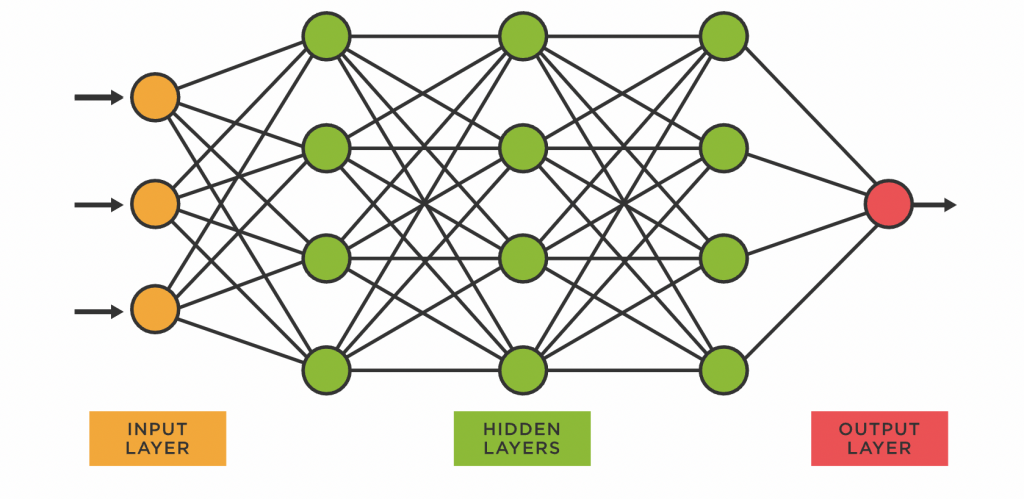
\includegraphics[width=1\linewidth]{chapters/PP/assets/R.png}
	\caption{Mạng nơ-ron nhân tạo nhiều lớp}
\end{figure}

\subsubsection*{Nguyên lý hoạt động:}

Quá trình xử lý dữ liệu trong MLP được chia thành hai giai đoạn chính: lan truyền tiến (forward propagation) và lan truyền ngược (backpropagation). Trong giai đoạn lan truyền tiến, dữ liệu đầu vào được truyền từ tầng đầu vào qua các tầng ẩn tới tầng đầu ra. Mỗi nơ-ron thực hiện phép biến đổi tuyến tính với trọng số và hệ số dịch như sau:

\[
z^{(l)} = W^{(l)} a^{(l-1)} + b^{(l)}, \quad a^{(l)} = \phi(z^{(l)})
\]

Trong đó:
\begin{itemize}
	\item $W^{(l)}$ là ma trận trọng số của tầng $l$
	\item $b^{(l)}$ là vector hệ số dịch (bias)
	\item $a^{(l-1)}$ là đầu ra của tầng trước
	\item $\phi$ là hàm kích hoạt phi tuyến
\end{itemize}

Sau khi đầu ra cuối cùng được tính toán, hàm mất mát (loss function) sẽ đo độ sai lệch giữa đầu ra dự đoán và nhãn thực tế. Hàm mất mát phổ biến trong bài toán phân loại là hàm cross-entropy, trong khi bài toán hồi quy thường dùng hàm MSE (Mean Squared Error).

Để cập nhật trọng số nhằm giảm sai số, thuật toán lan truyền ngược được sử dụng. Dựa trên đạo hàm của hàm mất mát đối với các trọng số, ta cập nhật từng trọng số theo hướng giảm gradient:

\[
W^{(l)} \leftarrow W^{(l)} - \eta \frac{\partial L}{\partial W^{(l)}}
\]

Trong đó $\eta$ là tốc độ học (learning rate), quyết định mức độ điều chỉnh sau mỗi lần cập nhật. Việc cập nhật có thể được thực hiện bằng nhiều thuật toán tối ưu khác nhau như Gradient Descent, Stochastic Gradient Descent (SGD), hay Adam — một phương pháp hiện đại và phổ biến vì khả năng hội tụ nhanh và ổn định.

\subsubsection*{Vai trò của hàm kích hoạt và khả năng biểu diễn phi tuyến}

Một điểm then chốt trong kiến trúc của MLP là việc sử dụng các hàm kích hoạt phi tuyến. Nếu toàn bộ mạng chỉ bao gồm các phép biến đổi tuyến tính, thì dù có nhiều tầng cũng không thể biểu diễn được hàm phi tuyến phức tạp. Hàm kích hoạt giúp mạng "bẻ cong" không gian đặc trưng, từ đó học được các mối quan hệ phức tạp trong dữ liệu.

Một số hàm kích hoạt phổ biến như:

\begin{itemize}
	\item \textbf{Sigmoid:} thích hợp cho đầu ra nhị phân nhưng dễ bị "vanishing gradient".
	\item \textbf{Tanh:} cải tiến so với sigmoid do có đầu ra đối xứng quanh 0, nhưng vẫn bị mất gradient ở biên.
	\item \textbf{ReLU:} đơn giản và hiệu quả, giúp giải quyết vấn đề mất gradient, tuy nhiên có thể bị "chết nơ-ron" nếu giá trị đầu vào âm liên tục.
	\item \textbf{Leaky ReLU:} một biến thể của ReLU có thể giải quyết vấn đề chết nơ-ron bằng cách cho phép gradient nhỏ hơn 0 ở phía âm.
\end{itemize}

Nhờ vào các hàm kích hoạt này, MLP có thể xấp xỉ bất kỳ hàm liên tục nào, theo định lý xấp xỉ phổ quát (Universal Approximation Theorem), nếu được cung cấp đủ nơ-ron và dữ liệu huấn luyện phù hợp.

Trong khi các phương pháp hồi quy tuyến tính hoặc cây quyết định có thể tốt với các mối quan hệ đơn giản hoặc có cấu trúc rõ ràng, MLP có thể học được các mối quan hệ không tuyến tính mà các phương pháp này không thể mô phỏng được. Điều này đặc biệt quan trọng trong dự báo giá nhà, vì giá trị bất động sản thường bị ảnh hưởng bởi nhiều yếu tố phức tạp, chẳng hạn như vị trí, kích thước, tình trạng tài chính của người mua, hoặc các yếu tố kinh tế vĩ mô mà không thể dễ dàng mô hình hóa bằng các phương pháp thông thường.

Với khả năng xấp xỉ các hàm phi tuyến, MLP có thể nắm bắt các mẫu dữ liệu phức tạp và linh hoạt hơn, đặc biệt khi dữ liệu huấn luyện có nhiều đặc trưng và mối quan hệ giữa chúng không phải là tuyến tính. Đột phá của MLP so với các phương pháp truyền thống là khả năng học từ dữ liệu mà không cần phải đưa ra giả định về mối quan hệ giữa các đặc trưng. MLP có thể tự động tìm ra các mối quan hệ phi tuyến, điều mà các mô hình hồi quy tuyến tính không thể thực hiện, từ đó nâng cao độ chính xác của dự báo giá nhà, đặc biệt trong các trường hợp có sự thay đổi hoặc biến động mạnh trong các yếu tố ảnh hưởng.

\section{Xây dựng mô hình dự đoán}

Sau khi hoàn tất bước tiền xử lý dữ liệu, tập dữ liệu được chia thành hai phần: tập huấn luyện (training set) và tập kiểm tra (test set) theo tỷ lệ 80:20. Việc phân chia này nhằm đảm bảo mô hình được đánh giá trên dữ liệu chưa từng thấy, từ đó phản ánh chính xác khả năng tổng quát hóa.

\begin{figure}[h!]
	\centering
	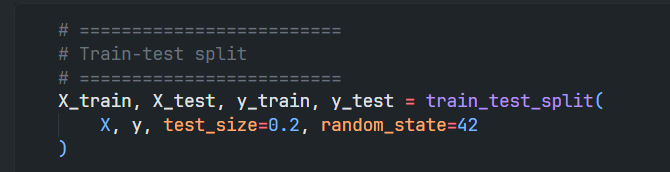
\includegraphics[width=1\linewidth]{chapters/Implement/ttsplit.png}
	\caption{Chia tập dữ liệu Train/Test}
\end{figure}

Mặc dù các đặc trưng trong tập dữ liệu đều ở dạng số, nhưng chúng có sự khác biệt lớn về thang đo. Điều này có thể ảnh hưởng tiêu cực đến hiệu quả của một số mô hình, đặc biệt là các mô hình tuyến tính.

Do đó, kỹ thuật chuẩn hóa dữ liệu \textbf{StandardScaler} được sử dụng để đưa các đặc trưng về cùng một phân phối với trung bình bằng 0 và độ lệch chuẩn bằng 1. Việc chuẩn hóa giúp cải thiện tốc độ hội tụ và độ ổn định trong quá trình huấn luyện.

\begin{figure}[H]
	\centering
	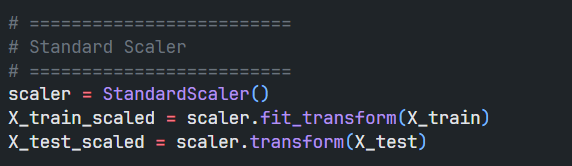
\includegraphics[width=1\linewidth]{chapters/Implement/scale.png}
	\caption{Chuẩn hóa dữ liệu với StandardScaler}
\end{figure}

Sau khi chuẩn bị dữ liệu, các mô hình được huấn luyện và đánh giá như sau:

\subsection{Hồi quy tuyến tính}

Mô hình hồi quy tuyến tính được huấn luyện trên dữ liệu đã được chuẩn hóa. Đây là mô hình cơ sở (baseline) nhằm thiết lập một mức tham chiếu cho hiệu suất của các mô hình phức tạp hơn.

\begin{figure}[H]
	\centering
	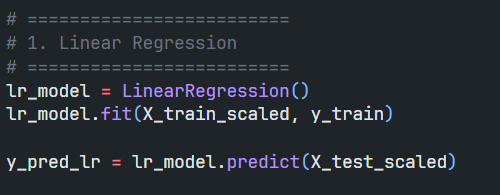
\includegraphics[width=0.5\textwidth]{chapters/Implement/linear.png}
	\caption{Mô hình hồi quy tuyến tính}
\end{figure}

\subsection{Random Forest}

Đối với mô hình Random Forest, nhóm sử dụng phương pháp \textbf{GridSearchCV} để tìm kiếm bộ siêu tham số tối ưu. Việc này giúp cải thiện hiệu suất mô hình một cách đáng kể.

Các siêu tham số được tinh chỉnh bao gồm:

\begin{itemize}
	\item \textbf{n\_estimators}: số lượng cây trong rừng
	\item \textbf{max\_depth}: độ sâu tối đa của cây
	\item \textbf{max\_features}: số đặc trưng được xét tại mỗi lần phân tách
	\item \textbf{min\_samples\_split}: số mẫu tối thiểu để chia node
	\item \textbf{min\_samples\_leaf}: số mẫu tối thiểu tại node lá
	\item \textbf{bootstrap}: sử dụng bootstrap sampling hay không
\end{itemize}

\begin{figure}[H]
	\centering
	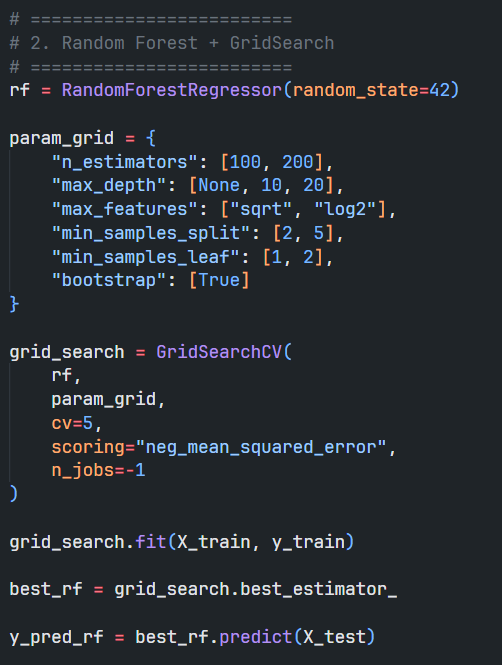
\includegraphics[width=0.8\linewidth]{chapters/Implement/GridCV.png}
	\caption{Tối ưu tham số với GridSearchCV}
\end{figure}

Sau quá trình tìm kiếm, mô hình thu được bộ tham số tối ưu giúp đạt hiệu suất tốt nhất trên tập validation.

\begin{figure}[H]
	\centering
	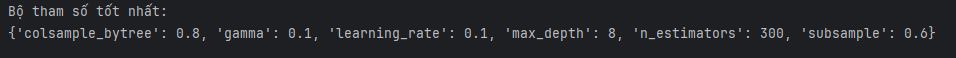
\includegraphics[width=0.8\linewidth]{chapters/Implement/BestParam.png}
	\caption{Bộ tham số tối ưu}
\end{figure}


\subsection{XGBoost}
Mô hình XGBoost được xây dựng và tối ưu hóa siêu tham số thông qua thuật toán tìm kiếm dạng lưới \texttt{GridSearchCV}. Quá trình này được kết hợp với phương pháp kiểm định chéo và sử dụng thang đo sai số toàn phương trung bình (Mean Squared Error - MSE) làm hàm mục tiêu đánh giá. 

Không gian tìm kiếm được thiết lập với các tham số cụ thể như sau:
\begin{itemize}
	\item \textbf{n\_estimators} (Tập giá trị thử nghiệm: \texttt{[100, 200, 300]}): Số lượng cây quyết định được xây dựng. Mỗi cây mới sẽ học cách bù đắp sai số cho các cây trước đó.
	
	\item \textbf{learning\_rate} (Tập giá trị thử nghiệm: \texttt{[0.01, 0.1]}): Điều chỉnh mức độ ảnh hưởng của mỗi cây mới lên mô hình cuối cùng. Giá trị nhỏ giúp mô hình hội tụ ổn định hơn và giảm thiểu rủi ro quá khớp (overfitting).
	
	\item \textbf{max\_depth} (Tập giá trị thử nghiệm: \texttt{[6, 8, 10]}): Chiều sâu tối đa của mỗi cây. Cây càng sâu càng nắm bắt được các quan hệ phi tuyến phức tạp, nhưng đồng thời làm tăng nguy cơ overfitting.
	
	\item \textbf{subsample} (Tập giá trị thử nghiệm: \texttt{[0.6, 0.8, 1.0]}): Tỷ lệ lấy mẫu ngẫu nhiên từ tập dữ liệu huấn luyện để xây dựng từng cây. Đặt giá trị nhỏ hơn 1 đóng vai trò như một kỹ thuật regularization.
	
	\item \textbf{colsample\_bytree} (Tập giá trị thử nghiệm: \texttt{[0.7, 0.8, 1.0]}): Tỷ lệ đặc trưng (features) được chọn ngẫu nhiên để huấn luyện tại mỗi cây, giúp các cây trong mô hình đa dạng hơn.
	
	\item \textbf{gamma} (Tập giá trị thử nghiệm: \texttt{[0.1, 0.3, 0.5]}): Ngưỡng giảm hàm mất mát tối thiểu yêu cầu để một node tiếp tục được phân nhánh. Đây là tham số quan trọng để kiểm soát độ phức tạp của cấu trúc cây.
\end{itemize}

% TODO: \usepackage{graphicx} required
\begin{figure}[H]
	\centering
	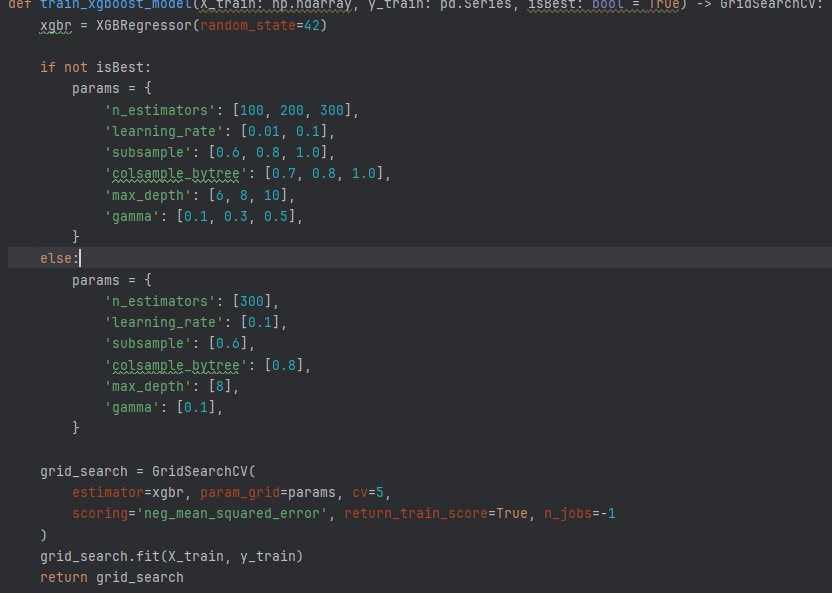
\includegraphics[width=0.8\linewidth]{chapters/Implement/CauhinhGrid}
	\caption{Cấu hình không gian tìm kiếm GridSearchCV cho XGBoost}
	\label{fig:cauhinhgrid}
\end{figure}

Sau khi rà soát toàn bộ các tổ hợp trong không gian siêu tham số, thuật toán đã hội tụ và xác định được bộ tham số tối ưu nhất, giúp mô hình đạt sai số thấp nhất trên tập kiểm định chéo. Kết quả bộ tham số tốt nhất được thể hiện như sau:

% TODO: \usepackage{graphicx} required
\begin{figure}[H]
	\centering
	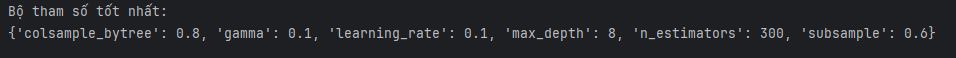
\includegraphics[width=0.8\linewidth]{chapters/Implement/BestParam}
	\caption{Bộ tham số tốt nhất cho mô hình}
	\label{fig:cauhinhgrid}
\end{figure}


\subsection{Mạng Nơ-ron nhiều lớp}
Ta tiến hành sử dụng phương pháp Nơ-ron nhiều lớp với cấu trúc như trong hình 5.8.
% TODO: \usepackage{graphicx} required
\begin{figure}[H]
	\centering
	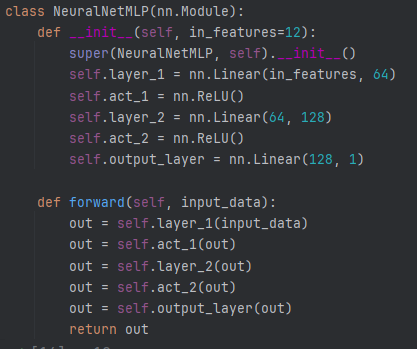
\includegraphics[width=0.6\linewidth]{chapters/Implement/MLP}
	\caption{Phương pháp mạng Nơ-ron nhiều lớp}
	\label{fig:mlp}
\end{figure}
Ta tiến hành huấn luyện mô hình với các tham số huấn luyện: 
\begin{itemize}
	\item Learning rate: 0.001
	\item Hàm mất mát: MSE
	\item Hàm tối ưu: Adam
	\item Số epoch: 35
\end{itemize}
Sau khi huấn luyện, ta tiến hành vẽ đồ thị mất mát. Thông qua đồ thị cho thấy cả Train Loss và Validation Loss đều giảm dần theo số epoch, với Train Loss giảm nhanh hơn trong 10 epoch đầu, sau đó cả hai đường ổn định từ epoch 20. Validation Loss luôn cao hơn Train Loss nhưng khoảng cách không lớn, chứng tỏ mô hình không bị overfitting nghiêm trọng. Đến khoảng 30-35 epoch, cả hai đường gần như không giảm thêm, đạt điểm hội tụ.
% TODO: \usepackage{graphicx} required
\begin{figure}[H]
	\centering
	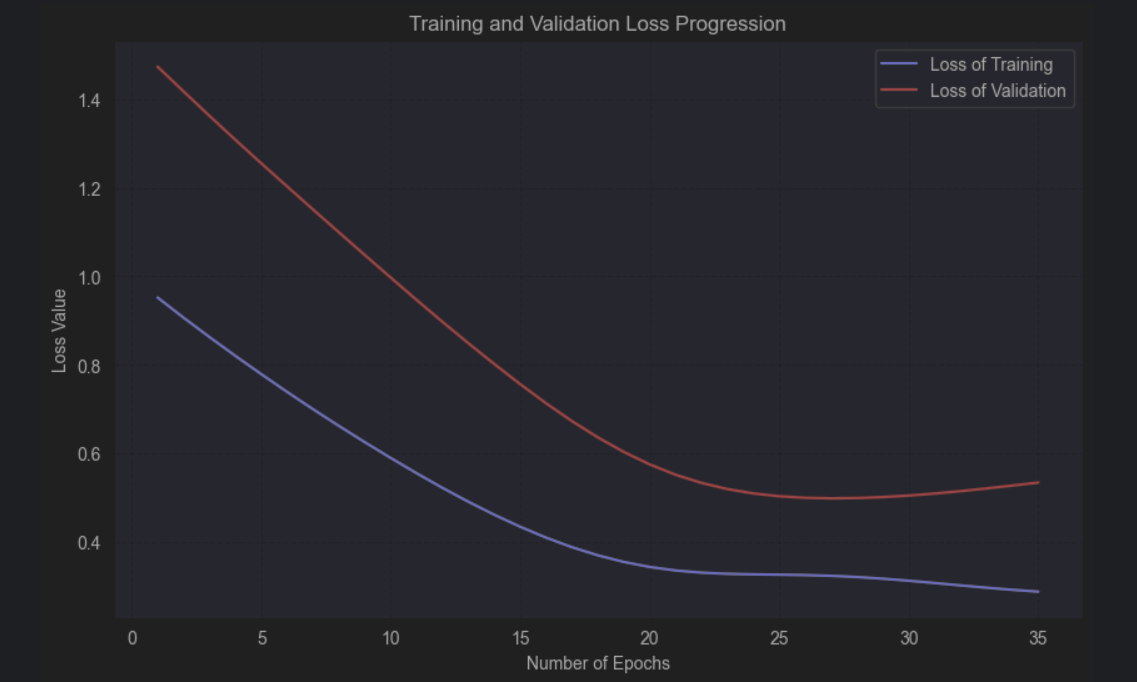
\includegraphics[width=0.8\linewidth]{chapters/Implement/Loss}
	\caption{Đồ thị mất mát}
	\label{fig:loss}
\end{figure}

\section{Đánh giá mô hình dự đoán}

\subsection{Các Phương pháp Đánh giá Hiệu quả Mô hình}

Để đánh giá hiệu quả của các mô hình học máy, bốn chỉ số phổ biến được sử dụng như sau:

\begin{itemize}
    \item \textbf{RMSE (Root Mean Square Error)}:
    \[
    RMSE = \sqrt{\frac{1}{n} \sum_{i=1}^{n} (y_i - \hat{y}_i)^2}
    \]

    \item \textbf{RRMSE (Relative RMSE)}:
    \[
    RRMSE = \frac{RMSE}{\overline{y}}
    \]

    \item \textbf{R-squared ($R^2$)}:
    \[
    R^2 = 1 - \frac{\sum_{i=1}^{n}(y_i - \hat{y}_i)^2}{\sum_{i=1}^{n}(y_i - \overline{y})^2}
    \]

    \item \textbf{MAE (Mean Absolute Error)}:
    \[
    MAE = \frac{1}{n} \sum_{i=1}^{n} |y_i - \hat{y}_i|
    \]
\end{itemize}

\subsection{Kết quả đánh giá}

Sau khi huấn luyện, nhóm thu được các chỉ số đánh giá như sau:

\begin{table}[H]
\centering
\caption{Các chỉ số đánh giá hiệu suất mô hình}
\begin{tabular}{|c|c|c|c|c|}
\hline
\textbf{Phương Pháp} & \textbf{RMSE} & \textbf{RRMSE} & \(\mathbf{R}^2\) & \textbf{MAE} \\
\hline
Linear Regression & 1,324,506.96 & 0.2645 & 0.653 & 970,043.40 \\
\hline
Random Forest & 1,400,619.50 & 0.2797 & 0.612 & 1,010,525.30 \\
\hline
XG\_Boost & 1,352,015.72 & 0.27 & 0.64 & 976,624.56 \\
\hline
Mạng Nơ-ron & 1,347,227.33 &0.27 & 0.64 & 956,810.86 \\
\hline
\end{tabular}
\end{table}

Dựa trên kết quả thu được, có thể rút ra các nhận xét chi tiết sau:

\begin{itemize}
	\item Mô hình \textbf{Hồi quy tuyến tính (Linear Regression)} đạt hiệu suất tổng thể tốt nhất dựa trên chỉ số RMSE thấp nhất ($1,324,506.96$) và hệ số xác định $R^2$ cao nhất ($0.653$). Điều này cho thấy tập dữ liệu có xu hướng phân bố tuyến tính khá mạnh, giúp một phương pháp cơ bản phát huy tối đa sức mạnh mà không gặp tình trạng quá khớp (overfitting).
	
	\item \textbf{Mạng Nơ-ron (MLP)} và \textbf{XGBoost} bám sát ngay sau với mức hiệu năng vô cùng ổn định ($R^2$ đều đạt mức $0.64$). Đáng chú ý, Mạng Nơ-ron lại là mô hình sở hữu sai số tuyệt đối trung bình (MAE) thấp nhất ($956,810.86$). Điều này chứng tỏ MLP có khả năng dự đoán các mức giá nhà thông thường rất sát với thực tế, dù thỉnh thoảng nhạy cảm với các điểm dị biệt (outliers) khiến chỉ số RMSE bị đẩy lên cao hơn so với Hồi quy tuyến tính.
	
	\item Mô hình \textbf{Random Forest} thể hiện hiệu suất kém nhất trong cả bốn phương pháp. Mặc dù là một thuật toán mạnh về khả năng mô hình hóa quan hệ phi tuyến, nhưng đối với tập dữ liệu này, thuật toán cây phân quyết định không mang lại hiệu quả, dẫn đến các chỉ số sai số cao nhất.
\end{itemize}

\textbf{Kết luận:} Dữ liệu trong bài toán mang đậm tính chất tuyến tính, do đó mô hình Hồi quy tuyến tính lại trở thành lựa chọn an toàn và hiệu quả nhất về mặt tổng thể. Tuy nhiên, nếu ưu tiên độ chính xác trên trung bình (dựa theo MAE), Mạng Nơ-ron nhiều lớp hoàn toàn là một giải pháp dự đoán đáng tin cậy.

\subsection{Đồ thị đánh giá}

Để trực quan hóa hiệu quả mô hình, nhóm sử dụng ba loại biểu đồ:

\begin{itemize}
    \item \textbf{Predictions vs Actual}: đánh giá độ chính xác tổng thể
    \item \textbf{Residuals vs Predicted}: kiểm tra lỗi hệ thống
    \item \textbf{Distribution of Residuals}: đánh giá phân phối sai số
\end{itemize}

\begin{figure}[H]
    \centering
    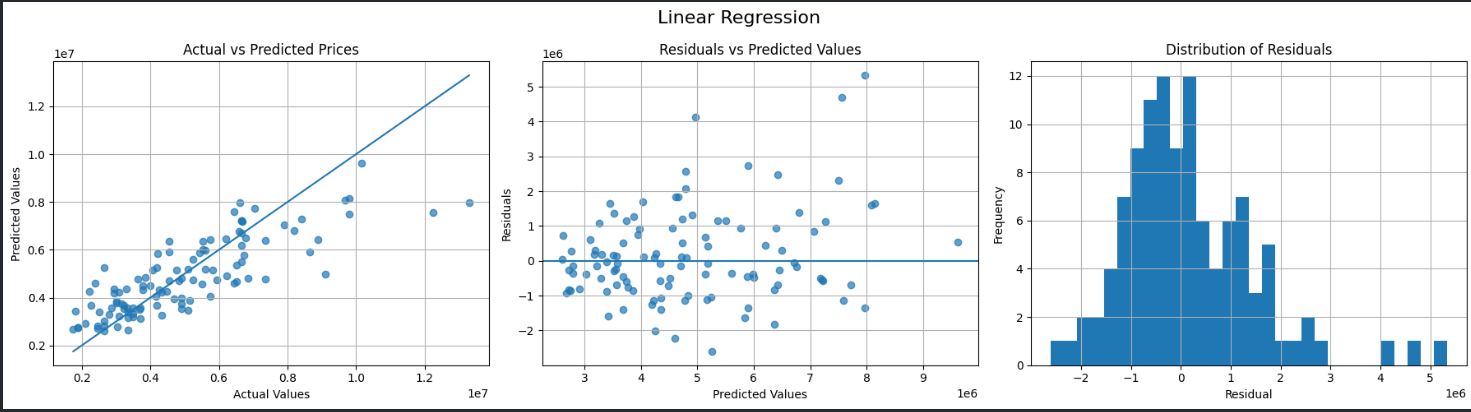
\includegraphics[width=0.95\textwidth]{chapters/Implement/linear_regression.png}
    \caption{Linear Regression: (a) Predictions vs Actual, (b) Residuals vs Predictions, (c) Distribution of Residuals}
    \label{fig:linear_eval}
\end{figure}

\begin{figure}[H]
    \centering
    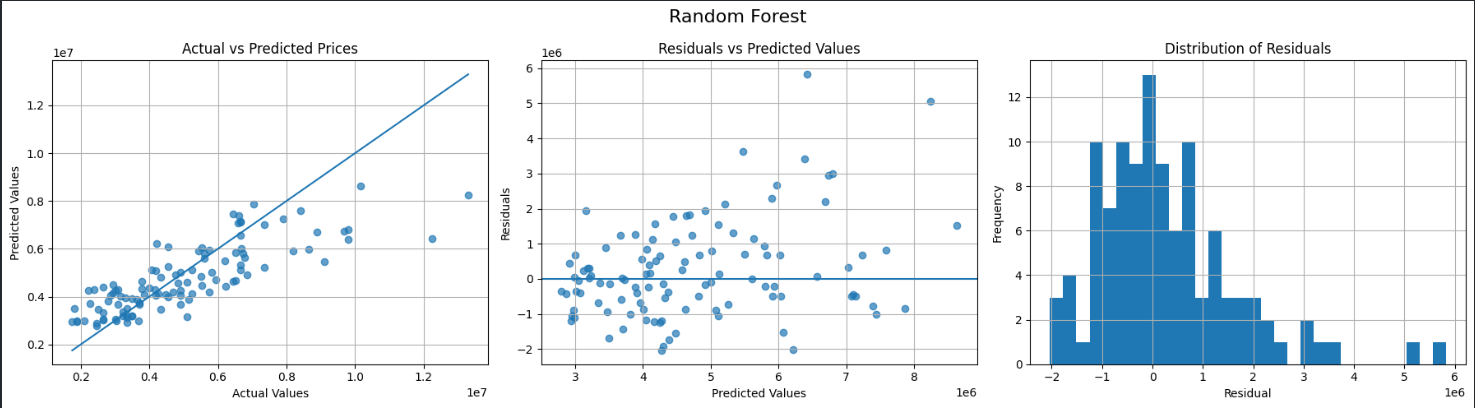
\includegraphics[width=0.95\textwidth]{chapters/Implement/random_forest.png}
    \caption{Random Forest: (a) Predictions vs Actual, (b) Residuals vs Predictions, (c) Distribution of Residuals}
    \label{fig:rf_eval}
\end{figure}

\begin{figure}[H]
	\centering
	\caption{XGBoost}
	
	\begin{minipage}{0.32\textwidth}
		\centering
		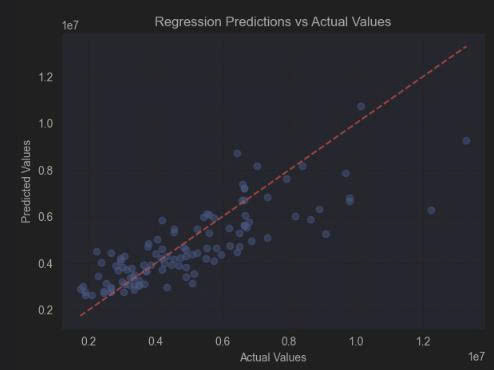
\includegraphics[width=\linewidth, height=6cm]{chapters/Preprocessing/images/xgb1.jpg}
		\textbf{(a) Predictions vs Actual}
		\label{fig:xgb_pred_vs_actual}
	\end{minipage}
	\hfill
	\begin{minipage}{0.32\textwidth}
		\centering
		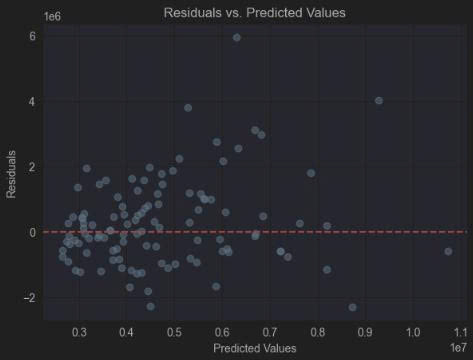
\includegraphics[width=\linewidth, height=6cm]{chapters/Preprocessing/images/xgb2.jpg}
		\textbf{(b) Residuals vs Predictions}
		\label{fig:xgb_residuals_vs_pred}
	\end{minipage}
	\hfill
	\begin{minipage}{0.32\textwidth}
		\centering
		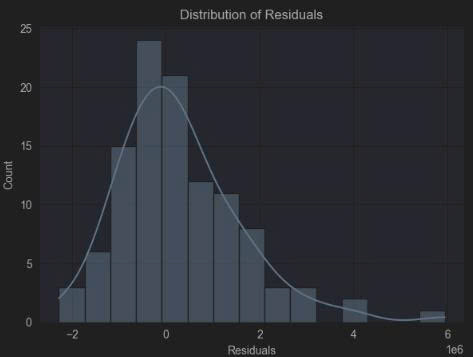
\includegraphics[width=\linewidth, height=6cm]{chapters/Preprocessing/images/xgb3.jpg}
		\textbf{(c) Distribution of Residuals}
		\label{fig:xgb_residuals_dist}
	\end{minipage}
\end{figure}


\begin{figure}[H]
	\centering
	\caption{Mạng Nơ-ron nhiều lớp}
	
	\begin{minipage}{0.32\textwidth}
		\centering
		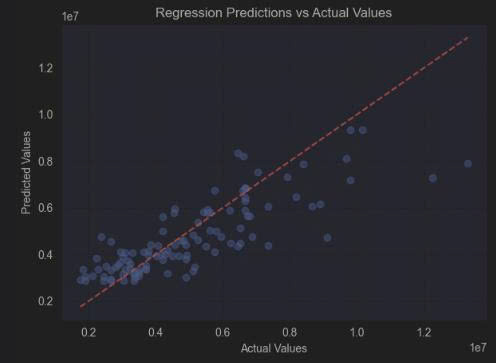
\includegraphics[width=\linewidth, height=6cm]{chapters/Preprocessing/images/mlp1.jpg}
		
		\textbf{(a) Regression Predictions vs Actual Values}
		\label{fig:regression}
	\end{minipage}
	\hfill
	\begin{minipage}{0.32\textwidth}
		\centering
		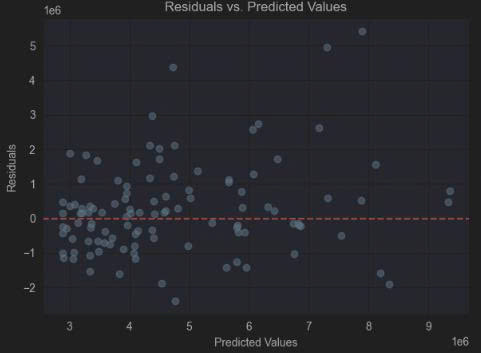
\includegraphics[width=\linewidth, height=6cm]{chapters/Preprocessing/images/mlp2.jpg}
		
		\textbf{(b) Residuals vs. Predicted Values}
		\label{fig:residuals_vs_pred}
	\end{minipage}
	\hfill
	\begin{minipage}{0.32\textwidth}
		\centering
		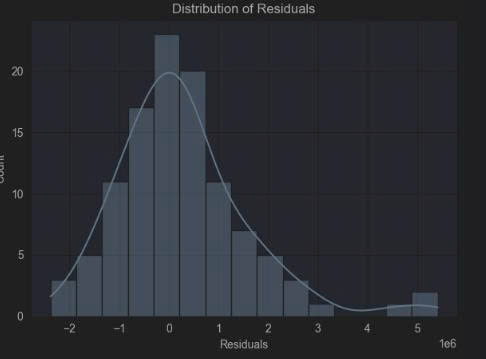
\includegraphics[width=\linewidth, height=6cm]{chapters/Preprocessing/images/mlp3.jpg}
		
		\textbf{(c) Distribution of Residuals}
		\label{fig:residual_distribution}
	\end{minipage}
\end{figure}

Từ các biểu đồ phân tích và giá trị dự đoán, có thể nhận thấy:

\begin{itemize}
	\item Với \textbf{Linear Regression}, các điểm dữ liệu phân bố khá sát đường lý tưởng $y = \hat{y}$. Phần dư phân bố ngẫu nhiên đều quanh trục 0 và biểu đồ phân phối phần dư có dạng hình quả chuông gần với phân phối chuẩn nhất, cho thấy mô hình dự đoán rất đồng đều và ổn định.
	
	\item Với \textbf{Random Forest}, độ phân tán của các điểm lớn hơn rõ rệt, đặc biệt phần dư có xu hướng loe rộng ra ở phân khúc các căn nhà có giá trị cao. Phân phối phần dư có xu hướng dẹt hơn, minh chứng cho việc mô hình gặp khó khăn và sai số lớn hơn so với mô hình tuyến tính.
	
	\item Với \textbf{XGBoost}, biểu đồ cho thấy sự cải thiện đáng kể so với Random Forest khi các điểm dự đoán bám sát đường lý tưởng hơn. Tuy nhiên, ở vùng giá trị cực đại, phần dư vẫn xuất hiện sự phân tán nhất định, chưa duy trì được độ hội tụ xuyên suốt như Linear Regression.
	
	\item Với \textbf{Mạng Nơ-ron (MLP)}, mật độ các điểm dữ liệu tập trung cực kỳ dày đặc và bám rất sát đường lý tưởng ở các phân khúc giá trung bình và thấp (phản ánh đúng việc mô hình đạt chỉ số MAE thấp nhất). Tuy nhiên, đồ thị phần dư cũng bộc lộ rõ một vài điểm dị biệt nằm rải rác khá xa trục 0, giải thích nguyên nhân chỉ số RMSE bị phạt nặng và cao hơn so với Hồi quy tuyến tính.
\end{itemize}

\subsection{Kết luận}

Thông qua quá trình huấn luyện, tối ưu hóa siêu tham số và đánh giá trực quan, nhóm có thể kết luận rằng \textbf{Hồi quy tuyến tính (Linear Regression)} là lựa chọn phù hợp và tối ưu nhất cho bài toán dự đoán giá nhà trên tập dữ liệu này. Nguyên nhân cốt lõi là do dữ liệu đầu vào thể hiện xu hướng tuyến tính rõ rệt, giúp một phương pháp thống kê cơ bản phát huy tối đa hiệu năng (RMSE thấp nhất, $R^2$ cao nhất), đồng thời tiết kiệm tuyệt đối chi phí tính toán.

Bên cạnh đó, \textbf{Mạng Nơ-ron nhiều lớp (MLP)} nổi lên như một giải pháp cực kỳ tiềm năng nếu hệ thống triển khai thực tế ưu tiên sai số tuyệt đối thấp nhất cho các căn nhà phổ thông (chỉ số MAE tốt nhất).

Ngược lại, các mô hình học máy theo dạng tập hợp phức tạp như Random Forest hay XGBoost lại không mang lại sự đột phá đáng kể về mặt độ chính xác, thậm chí tiêu tốn nhiều tài nguyên hơn cho việc tìm kiếm siêu tham số, do đó không phải là hướng tiếp cận hiệu quả nhất trong bối cảnh dữ liệu hiện tại.

\section{Tổng Kết}
Trong bài tập lớn lần này, nhóm đã tiến hành đầy đủ các bước trong quy trình khai phá tri thức nhằm tìm ra mô hình phù hợp nhất để giải quyết bài toán dự đoán giá nhà, sử dụng tập dữ liệu gồm 545 ngôi nhà với các thuộc tính đặc trưng có giá trị cho quá trình huấn luyện.

Từ dữ liệu thô thu thập được trên nền tảng Kaggle, nhóm đã lần lượt thực hiện các bước: làm sạch dữ liệu, tích hợp dữ liệu, chọn lọc thuộc tính, chuyển đổi dữ liệu, khai phá dữ liệu, đánh giá mô hình và biểu diễn tri thức. Bốn phương pháp khai phá dữ liệu được áp dụng gồm: Hồi quy tuyến tính, Random Forest, XGBoost và mạng Nơ-ron nhiều lớp (Neural Network), nhằm so sánh và lựa chọn mô hình tối ưu.

Thông qua quá trình huấn luyện và đánh giá, cả bốn mô hình đều cho kết quả khả quan. Tuy nhiên, mô hình \textbf{Hồi quy tuyến tính (Linear Regression)} thể hiện hiệu năng tổng thể vượt trội nhất (đạt chỉ số RMSE thấp nhất và $R^2$ cao nhất). Điều này xuất phát từ việc các đặc trưng trong tập dữ liệu mang đậm tính chất tuyến tính, giúp một mô hình thống kê cơ bản phát huy tối đa sức mạnh, đảm bảo khả năng tổng quát hóa cao mà không bị rơi vào trạng thái quá khớp (overfitting). 

Bên cạnh đó, \textbf{Mạng Nơ-ron nhiều lớp (MLP)} cũng là một điểm sáng đáng ghi nhận khi đạt mức sai số tuyệt đối trung bình (MAE) thấp nhất trong cả bốn phương pháp, cho thấy khả năng dự đoán cực kỳ sát sao đối với các phân khúc nhà phổ thông. Mô hình \textbf{XGBoost} xếp ngay sau với sự hội tụ ổn định và độ tin cậy cao.

Tóm lại, để triển khai trong hệ thống dự đoán giá nhà thực tế, Hồi quy tuyến tính là lựa chọn ưu tiên hàng đầu nhờ sự cân bằng hoàn hảo giữa độ chính xác, chi phí tài nguyên tính toán thấp và tính dễ diễn giải. Nếu hệ thống đặc thù yêu cầu tối thiểu hóa sai số tuyệt đối trên từng căn nhà cụ thể, mạng Nơ-ron sẽ là một phương án triển khai xuất sắc.

\bibliographystyle{plain}
\nocite{*}

\end{document}
